\section{Orthogonal Terrains}
\label{sec:orthogonal_terrains}

In this section, we outline a construction of orthogonal terrains with arbitrary rational extrusion heights.
In our construction, the cross section at will always be on the $x-z$ plane.
This makes the analysis much simpler.
\graphicspath{{./figures/}}
\begin{figure}[!htb]
    \centering
    \subfloat[Orthogonal terrain.]{
        \includegraphics[width=0.4\linewidth]{figures/terrain.png}
        \label{fig:terrain}
    }%
    \subfloat[A column extrusion with heights $\{0,1,3,1,2,0\}$]{
        \def\svgwidth{0.6\textwidth}
        \input{./figures/column_extrusion.pdf_tex}%
        \label{fig:column_extrusion}
    }%
    \caption{}
\end{figure}%

To simplify the presentation, we will consider an uniform $X-Y$ grid,
with arbitrary rational extrusion heights corresponding to every grid square (Figure~\ref{fig:terrain}).
\begin{definition}
An $n\times m$ rational grid extrusion is a 3-dimensional structure,
whose projection onto the $x-y$ plane forms an unit grid of size $n\times m$.
In the 3-dimensional structure, the unit face corresponding to the location $(i.j)$,
exists at height $E_{i,j}$ (in the $z$ direction), where $E_{i,j}$ is a rational number.
\end{definition}
%In the case that $E_{i,j}$ is rational, we can simply scale down down our construction by an appropriate size, to obtain integer heights.

We consider each ''column'' of a given grid extrusion separately as an individual \emph{column extrusion}.
We will construct each of the $n$ columns independently (Figure~\ref{fig:level_shift}),
and attach them together with \emph{column connectors} (Figure~\ref{fig:column_connector}).

We begin by choosing an $2\varepsilon=1/K$ where $K$ is a positive integer.
This is chosen such that $E_{i,j}$ is an integral multiple of $2\varepsilon$ for all $i,j$.
Then we scale the entire construction up by a factor of $K$.

Given a strip of size $X\times T$, we will consider the evolution of a cross section of length $X$ evolving for time $T$.
%Imagine that there are $T = \frac Y\varepsilon$ time steps of length $\varepsilon$, over which the cross section evolves along the $y$-axis.

\subsection{Construction of Grid Extrusion}
\label{sec:construction}

We begin by choosing an $2\epsilon=1/K$ where $K$ is a positive integer.
This is chosen such that $E_{i,j}$ is an integral multiple of $2\epsilon$ for all $i,j$.
Then we scale the entire construction up by a factor of $K$.

Given a strip of size $X\times T$, we will consider the evolution of a cross section of length $X$ evolving for time $T$.
%Imagine that there are $T = \frac Y\epsilon$ time steps of length $\epsilon$, over which the cross section evolves along the $y$-axis.

\subsection{Construction of Column Extrusion by Level Shifting}
\label{sec:column_extrusion}

First, we consider a single column of the orthogonal terrain $\left\{ E_{i1}, E_{i2}, \cdots, E_{i,n} \right\}$.
We denote the column extrusion heights as $\left\{ H_1, H_2,\cdots H_n \right\}$, where $H_j = E_{i,j}$.
Consider the decomposition of $T$ into the following time intervals.% (parallel to the $x$-axis).
\begin{align}
    \label{eq:column_decomposition}
T = 1 + D_1  +  1 + D_2  +  1 + D_3  +\cdots\cdots +  1 + D_{m-1}  +  1
\end{align}
Here, the times corresponding to
\begin{itemize}
\item the $i^{th}$ 1 is realized as the surface at height $H_i$.
\item $D_i = \left| H_i-H_{i+1}\right|$ is realized as the transition between $H_i$ and $H_{i+1}$.  \end{itemize}

\graphicspath{{./figures/}}
\begin{figure}[htb]
    \def\svgwidth{1.0\textwidth}
    \input{./figures/level_shift_layers.pdf_tex}%
    \caption{
    Cross section change from level $i$ to $i+1$.
    The \emph{accordion segments} are separated for illlustration.
    In reality, the accordion is folded flat.
    The direction of horizontal and vertical segments are shown by purple and green arrows respectively.
    }
    \label{fig:level_shift_layers}
\end{figure}

\graphicspath{{./figures/level_shift/}}%
\begin{figure}[t!]%
    \centering
    \begingroup%
        \def\svgwidth{0.25\textwidth}
        \captionsetup[subfigure]{width=0.25\textwidth}
        \subfloat[Higher initial level. Top segment moves down.]{%
            \input{./figures/level_shift/column0.pdf_tex}
            \label{fig:level_shift0}
        }%
    \endgroup
    \subfloat[Two segments created. New segments are aligned with top segment, and move down. Vertical segments move inwards.] {%
        \def\svgwidth{0.24\textwidth}
        \input{./figures/level_shift/column1.pdf_tex}%
        \def\svgwidth{0.25\textwidth}
        \input{./figures/level_shift/column2.pdf_tex}%
        \label{fig:level_shift1}
    }%
    \def\svgwidth{0.25\textwidth}
    \subfloat[Two more segments created. Vertical segments reverse direction.] {%
        \input{./figures/level_shift/column3.pdf_tex}%
    %}%
        \def\svgwidth{0.27\textwidth}
    %\subfloat[] {
        \input{./figures/level_shift/column4.pdf_tex}%
    %}%
        \def\svgwidth{0.29\textwidth}
    %\subfloat[] {
        \input{./figures/level_shift/column5.pdf_tex}%
        \label{fig:level_shift2}
    }%

    \subfloat[Level shift completed with four new horizontal segments.] {%
        \def\svgwidth{0.29\textwidth}
        \input{./figures/level_shift/column6.pdf_tex}%
        \def\svgwidth{0.34\textwidth}
        \input{./figures/level_shift/column7.pdf_tex}%
        \label{fig:level_shift3}
    }%
    \begingroup
        \def\svgwidth{0.27\textwidth}
        \captionsetup[subfigure]{width=0.24\textwidth}
        \subfloat[Flat folded state.]{%
            \input{./figures/level_shift/column8.pdf_tex}%
            \label{fig:level_shift4}
        }%
    \endgroup%
    \caption{Level shifting gadget. The separation along the $Y$ direction illustrates the layering. The red line denotes the boundary of the cross section.}
    \label{fig:level_shift}
\end{figure}%
%

To construct the column, we will present a cross section sequence.
First, consider $H_i$, such that $H_{i+1} = H_i-2\epsilon\cdot d$.
Figure~\ref{fig:level_shift_layers} shows the cross section evolution.
This cross section comprises of a two vertical lines separated by a top horizontal line.
The vertical lines are connected to the top segment with
a sequence of $2k$ horizontal segments that \emph{accordion} back and forth.
During the $K$-interval, all segments move along the positive $y$ direction (Figure~\ref{fig:level_shift0}),to create the $i^{th}$ level.
Subsequently, during the level shift, all segments move in the $x-z$ plane (Figure~\ref{fig:level_shift1}~\ref{fig:level_shift2}).
\todo[inline]{$y$ movement}
\begin{lemma}
\label{lem:accordion_even}
The number of accordion folds during horizontal evolution (along the $y$ axis) must be even.
\end{lemma}


The top segment moves downwards in intervals of $2\epsilon$.
During this process, the horizontal segments move downwards continuously (Figure~\ref{fig:level_shift1}~\ref{fig:level_shift2}).
For the first $\epsilon$ time interval, a new horizontal downwards moving accordion segment of length zero is created at both accordions,
and the vertical segments move towards each other along the $x$-axis (Figure~\ref{fig:level_shift1}).
For the next $\epsilon$ time interval, similar (oppositely oriented) accordion segments are created at the lowest position.
This time, the vertical segments move outwards.
Overall, two sets of accordion segments on either side are added, and the height of the top segment decreases by $2\epsilon$.

In the case that $H_{i+1} = H_i+2\epsilon\cdot d$, the level up-shift is simply the down-shift evolution in reverse (Figure~\ref{fig:column_connector}).
This transition is only possible if the initial number of accordion segments in the $H_i$ cross section is at least $2d$.
Specifically, assuming that the minimum height is zero, we have the following lemma.
\begin{lemma}
\label{lem:layer_change}
If the number of accordion segments at level $H_i$ is $l_i$,
then the number of accordion segments after transitioning to level $H_{i+1}$ is $l_{i+1} = l_i - (H_{i+1}-H_i)/\epsilon$.
Specifically, if the number of layers at level $0$ is $l$, then the number of layers
at level $\max\left\{ H_i\right\}$ is $l - \max\left\{ H_i\right\}/\epsilon$.
\end{lemma}
\begin{corollary}
\label{cor:layer_limit}
Since the number of accordion segments can never be negative, the minimum number of layers at at level zero
is $L = \max\left\{ H_i\right\}/\epsilon$. This also ensures that every other level shift is also possible.
\end{corollary}
\begin{corollary}
\label{cor:column_cross_section_length}
The length of the cross section at a zero level is at least $1 + 2\cdot L\cdot \epsilon$.
So, the minimum possible length of the cross section under our construction is $1 + 2\cdot\max\left\{ H_i\right\}$.
\end{corollary}

This provides the minimum width of the strip required to construct a column extrusion.
Now, we can also calculate the length of the strip as the total time evolution required
$$ T = 1 + D_1  +  1 + D_2  +  1 + D_3  +\cdots\cdots +  1 + D_{m-1}  +  1 = m + \sum^{m-1}_{i=1} \left| H_{i+1}-H_i\right| $$

\begin{theorem}
\label{thm:column_extrusion}
A given column extrusion with heights $\left\{ H_1, H_2,\cdots H_n \right\}$, can be constructed from a strip of paper with size
$\left( 1 + 2\cdot\max\left\{ H_i\right\}\right)\times T$, where
$$T \ge \left( m + \sum\limits^{m-1}_{i=1} \left| H_{i+1}-H_i\right|\right)$$
\end{theorem}

\subsection{Multiple Column Extrusions form a Grid Extrusion}
\label{sec:grid_extrusion}

Now, we consider mutiple column extrusions evolving in parallel.
Henceforth, we will refer to the evolution of column cross sections along the $y$-axis
(the ''1''s in Equation~\ref{eq:column_decomposition} as \emph{horizontal evoluton}.
Meanwhile, a \emph{vertical transition} will refer to level shifting evolution in the $x-z$ plane.
Let $\mathcal C^{(i)}$ be a valid cross section evolution corresponding
to the $i^{th}$ column in the grid extrusion (as defined in Section~\ref{sec:column_extrusion}).
As before, for simplicity, we will assume that the minimum height in each column is zero $\left( i.e.\ \min_j\left\{ E_{i,j}\right\} = 0 \right)$.

\graphicspath{{./figures/up_down/}}%
\begin{figure}[ht!]%
    \centering
    \begingroup%
        \captionsetup[subfigure]{width=0.18\textwidth}
        \subfloat[Column starts at initial level $H_i$] {
            \def\svgwidth{0.22\textwidth}
            \input{./figures/up_down/up_down0.pdf_tex}%
            \label{fig:up_down0}
        }%
    \endgroup
    \begingroup%
        \captionsetup[subfigure]{width=0.44\textwidth}
        \subfloat[Two segments created. New segments are aligned with top segment, and move down.] {
            \def\svgwidth{0.205\textwidth}
            \input{./figures/up_down/up_down1.pdf_tex}%
        %}%
        %\subfloat[] {
            \def\svgwidth{0.215\textwidth}
            \input{./figures/up_down/up_down2.pdf_tex}%
            \label{fig:up_down1}
        }%
    \endgroup
    \begingroup%
        \captionsetup[subfigure]{width=0.2\textwidth}
        \subfloat[Segments reverse direction] {
            \def\svgwidth{0.22\textwidth}
            \input{./figures/up_down/up_down3.pdf_tex}%
            \label{fig:up_down2}
        }%
    \endgroup

    \begingroup%
        \captionsetup[subfigure]{width=0.55\textwidth}
        \subfloat[Cross section returns to initial state, and continues horizontal evolution.] {
            \def\svgwidth{0.28\textwidth}
            \input{./figures/up_down/up_down4.pdf_tex}%
        %}%
        %\subfloat[] {
            \def\svgwidth{0.31\textwidth}
            \input{./figures/up_down/up_down5.pdf_tex}%
            \label{fig:up_down3}
        }%
    \endgroup
    \begingroup%
        \captionsetup[subfigure]{width=0.27\textwidth}
        \subfloat[Flat folded state] {
            \def\svgwidth{0.27\textwidth}
            \input{./figures/up_down/up_down6.pdf_tex}%
            \label{fig:up_down4}
        }%
    \endgroup
    \caption{Up-down gadget. The separation along the $Y$ direction illustrates the layering. The red line denotes the boundary of the cross section.}
    \label{fig:up_down}
\end{figure}%
%

We consider the parallel evolution of each column extrusion $\mathcal C^{(i)}$.
\begin{itemize}
    \item During the horizontal evolution of row $j$, each $\mathcal C^{(i)}$ evolves along the positive $y$ direction for time $1$ at height $E_{i,j}$.
    \item During the vertical transition from row $j$ to $j+1$, each $\mathcal C^{(i)}$ evolves for time $ D_{ij} = \left| E_{i,j+1}-E_{i,j}\right|$.
\end{itemize}
Note that the vertical transition times are different for each $\mathcal C^{(i)}$.
Since we want to glue the sequence of $\left\{ \mathcal C^{(i)}\right\}$s, our constructions must have equal transition times.

\begin{definition}
\label{def:slowest_column}
We define the common transition time from row $j$ to row $j+1$ as
$$D_j = \max_j\left\{ D_{ij}\right\} = \max_j\left\{ \left| E_{i,j+1}-E_{i,j}\right|\right\}.$$
\end{definition}

So, the slowest column dictates the transition time, and the faster columns have to \emph{stall} for additional time.
To achieve this, we define an \emph{up-down} gadget, which is very similar to our original level shifting gadget.
This up-down gadget (Figure~\ref{fig:up_down}) evolves for $2\varepsilon$ time, but the height of the corresponding column remains unchanged.
This gadget starts at a height $H_i$, and for the first $\varepsilon$ time interval (Figure~\ref{fig:up_down1}),
evolves exactly the same way as the down-shift gadget (Figure~\ref{fig:level_shift1}).
For the second $\varepsilon$ time interval, the cross section evolves in reverse (Figure~\ref{fig:up_down2}),
back to it's original state at height $H_i$ (Figure~\ref{fig:up_down3}).

So, the vertical transition of $\mathcal C^{(i)}$ needs to use a total of $\left( D_j - D_{i,j}\right)/\left( 2\varepsilon\right)$
up-down gadgets (each gadget \emph{stalls} for $2\varepsilon$ time).
%Notice that this gadget requires at least one accordion segment. In fact, by Lemma~\ref{lem:accordion_even}, it requires two segments.
%Given the worst case scenario, where $E_{i,j}=E_{i,j+1}$ is the max height in column $i$,
We obtain the following primitive, as a consequence of Theorem~\ref{thm:column_extrusion}.

\begin{proposition}
\label{prop:accordion_layers}
%The number of accordion layers for column $i$ at its minium height is
%$L_i = 2 + \left( \max_j\left\{ E_{i,j}\right\} - \min_j\left\{ E_{i,j}\right\} \right)/\varepsilon$.
By Theorem~\ref{thm:column_extrusion}, the extrusion for column $i$ is constructed from a paper strip with size
$$\left( 1 + 2\cdot\max_j\left\{ E_{ij}\right\}\right)\times \left( m + \sum\limits^{m-1}_{j=1} D_j \right). $$
\end{proposition}

\subsection{Gluing Column Extrusions together with Strip Connectors}
\label{sec:strip_connectors}
Now that all the column extrusions $\left\{ \mathcal C^{(i)} \right\}$ have the same evolution time,
we would like to glue them together into a continuous strip of paper.
In order to achieve this, we consider the time-axis boundaries of $\mathcal C^{(i)}$ (red line in Figure~\ref{fig:level_shift},~\ref{fig:up_down}).
First, note that the boundaries always lie on the same plane, corresponding to the zero level.
We will constrain this to be on the plane $z=0$. Now, let us consider the motion of the boundary on this plane.

\graphicspath{{./figures/}}
\begin{wrapfigure}[16]{r}{0.27\textwidth}
    \vspace{-2.8em}
    \def\svgwidth{0.27\textwidth}
    \input{./figures/boundaries.pdf_tex}%
    \caption{Boundaries of adjacent column extrusions ($D_j = 8\varepsilon$). $\phi$ denotes a zero distance.}
    \label{fig:boundaries}
    %\vspace{-1.8em}
\end{wrapfigure}
\begin{itemize}
    \item During the horizontal evolution of any row $j$, both boundaries move along the positive $y$-axis with unit velocity
          (Figure~\ref{fig:level_shift0},~\ref{fig:level_shift3},~\ref{fig:level_shift4},~\ref{fig:up_down0},~\ref{fig:up_down3},~\ref{fig:up_down4}).
%\end{itemize}
%\begin{itemize}[resume, before = \vspace*{-\dimexpr\topsep+\partopsep\relax}]
    \item During the vertical transition from row $j$ to $j+1$, both boundaries move back and forth along the $x$-axis with unit velocity.
          (Figure~\ref{fig:level_shift1},~\ref{fig:level_shift2},~\ref{fig:up_down1},~\ref{fig:up_down2}).
          We can divide the vertial transition into $k = D_j/(2\varepsilon)$ intervals of length $2\varepsilon$.
          Each of these interval segments is either a up-shift, a down-shift, or a up-down gadget.
    \begin{itemize}
        \item In the first half of each interval ($\varepsilon$ time), the left and right boundaries move towards each other;
              i.e. the left boundary moves along the positive $x$-axis,
              and the right boundary moves along the negative $x$-axis for a distance of $\varepsilon$.
        \item In the second half of each interval, the left and right reverse velocites, and return to their original positions.
        \item After $D_j$ time, the boundaries return to their original positions, and resume their movement in the positive $y$ direction.
    \end{itemize}
\end{itemize}

We will attempt to construct a cross section sequence whose left and right boundaries
line up with the adjacent column extrusion boundaries shown in Figure~\ref{fig:boundaries}.
Notice that the distance between \emph{corresponding points} on the boundaries varies between $0$ and $2\varepsilon$.
So, the connector strip must have width at least $2\varepsilon$.

We outline a construction of a $2\varepsilon$ width strip, as shown in Figure~\ref{fig:connector_cross_section}.
During horizontal evolution, the cross section comprises of two vertical segments, each of length $\varepsilon$,
which move along the same trajectory in the positive $y$-direction
(during horizontal evolution Figure~\ref{fig:column_connector0},~\ref{fig:column_connector10}).
Now, consider a transition of length $D_j$ divided into intervals of length $2\varepsilon$,
each of which evolves according to Figure~\ref{fig:connector_cross_section}.
\begin{itemize}
    \item The vertical segments move outwards with unit velocity to match the outward moving boundaries of the adjacent strips.
          An upwards moving horizontal segment of length zero is created between the two existing segments (Figure~\ref{fig:column_connector1}).
\end{itemize}

\begin{itemize}[resume, before = \vspace*{-\dimexpr\topsep+\partopsep\relax}]
    \item After time $\varepsilon$, the length of the vertical segments become zero,
          and the horizontal segment spans the $2\varepsilon$ gap between the column boundaries (Figure~\ref{fig:column_connector2}).
          Notice that that the boundary of the connector maintains its $z$ coordinate (Figure~\ref{fig:connector_cross_section}).
    \item Then the connector segments reverse velocites, and retrace their path for $\varepsilon$ time (Figure~\ref{fig:column_connector3}),
          until the vertical segments become length $\varepsilon$, and the horizontal segment disappears (Figure~\ref{fig:column_connector4}).
    \item The entire process repeats $D_j/(2\varepsilon)$ times (Figure~\ref{fig:column_connector5},~\ref{fig:column_connector6},~\ref{fig:column_connector7}).
\end{itemize}

The completed connector gadget is shown in Figure~\ref{fig:column_connector8},~\ref{fig:column_connector9}.
We show the \emph{connector gadget} attched to an \emph{up-shift gadget} in Figure~\ref{fig:column_connector7},~\ref{fig:column_connector10}.
\graphicspath{{./figures/}}
\begin{figure}[!h]
    \def\svgwidth{1.0\textwidth}
    \input{./figures/connector_cross_section.pdf_tex}%
    \caption{
    Cross section evolution of column connector gadget.
    }
    \vspace{-1.5em}
    \label{fig:connector_cross_section}
\end{figure}

\begin{figure}[!htb]
\graphicspath{{figures/column_connector}}
    \centering
    \subfloat[Initial height.]{
        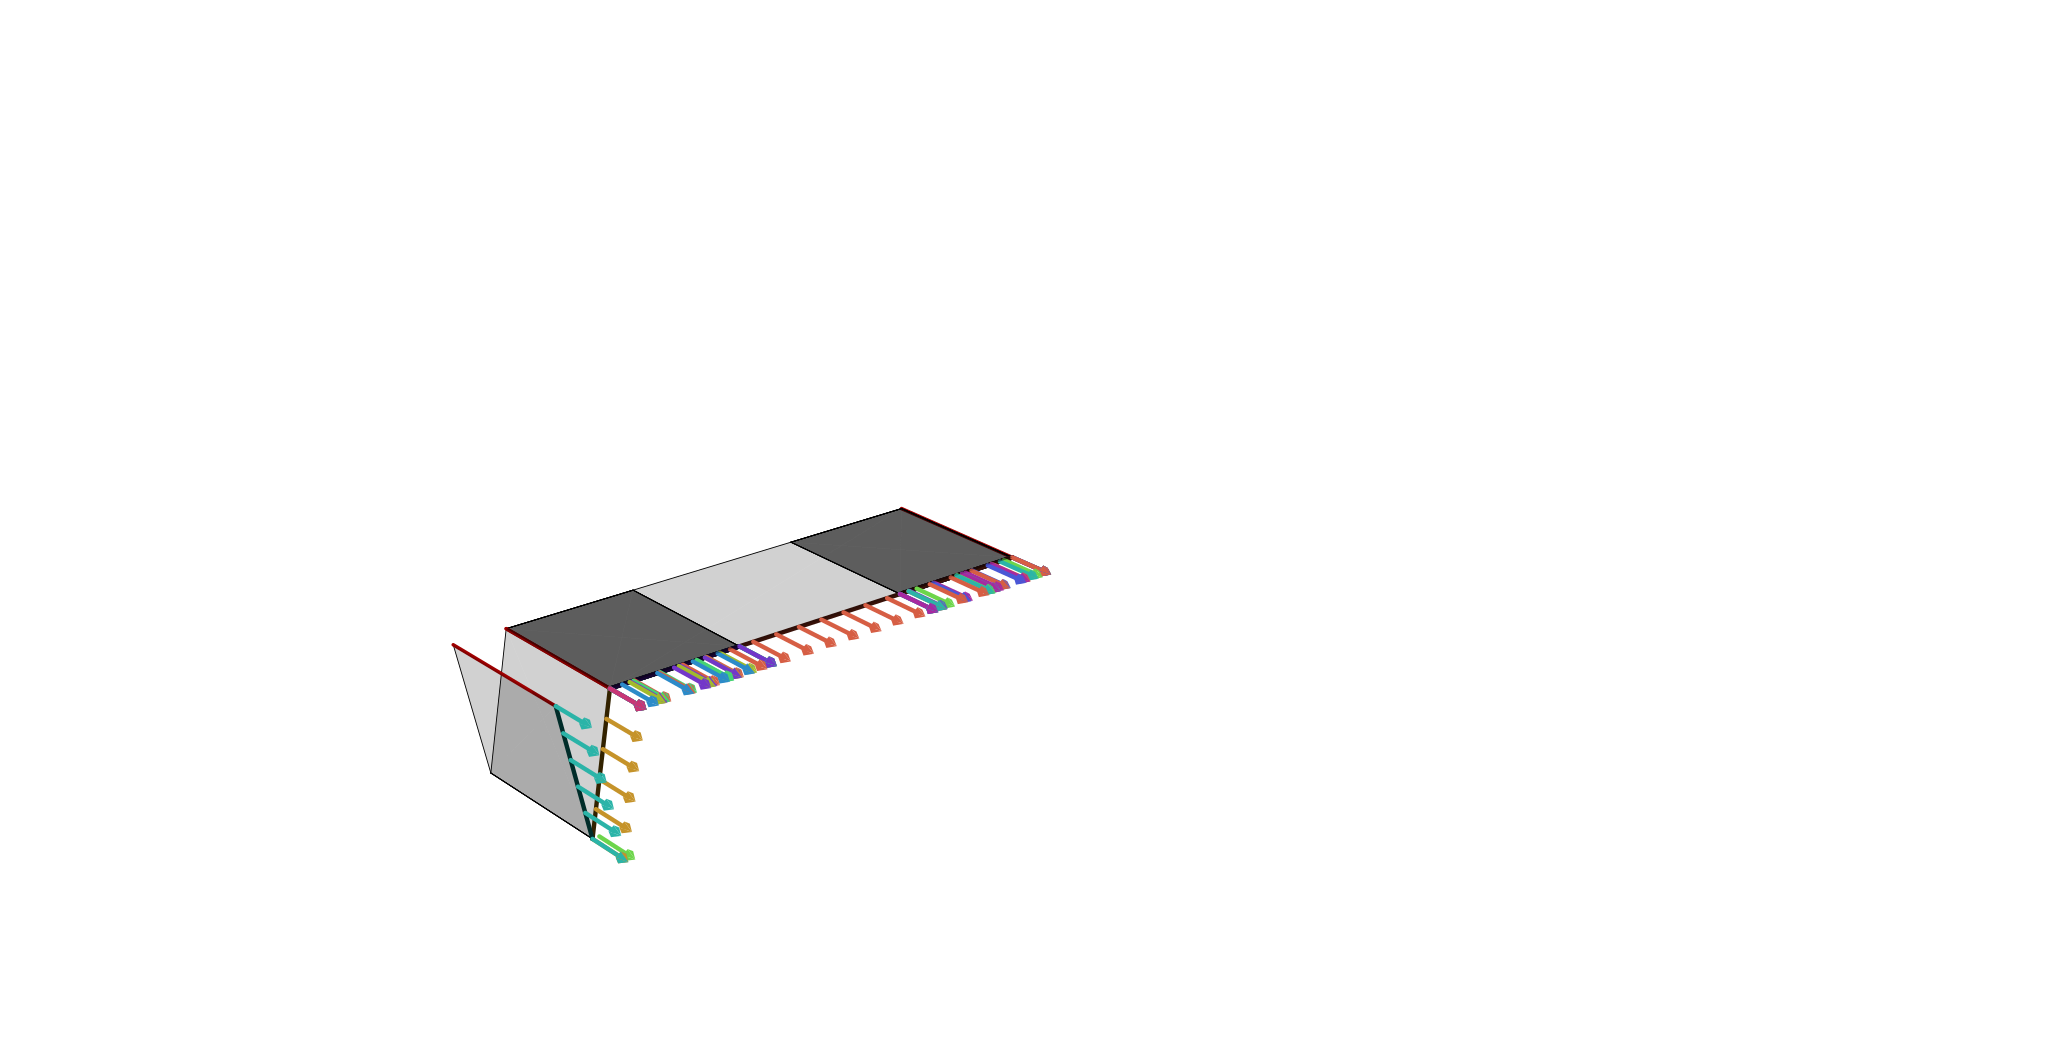
\includegraphics[width=0.23\textwidth]{figures/column_connector/column0.pdf}
    }%
    \subfloat[Connector moves outwards.]{
        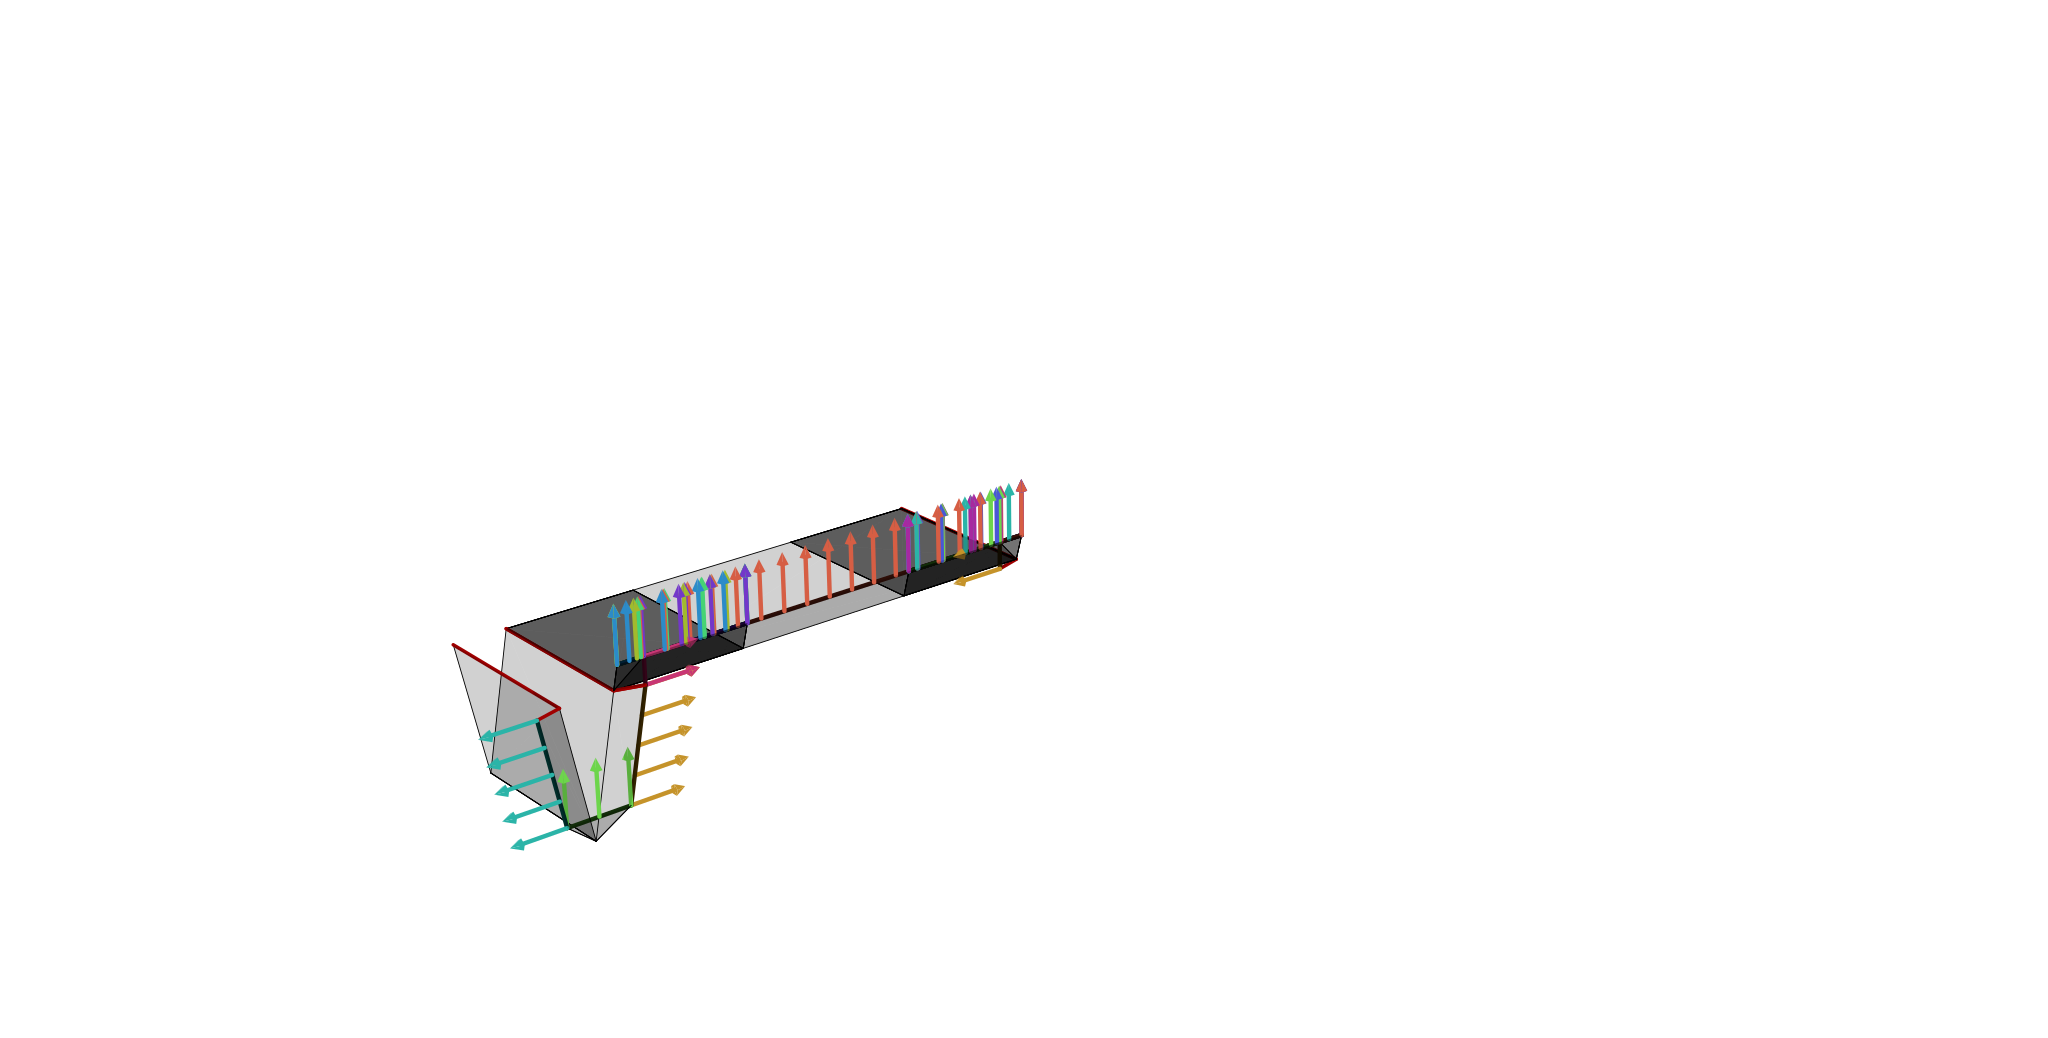
\includegraphics[width=0.21\textwidth]{figures/column_connector/column1.pdf}
    %}
    %\subfloat[]{
        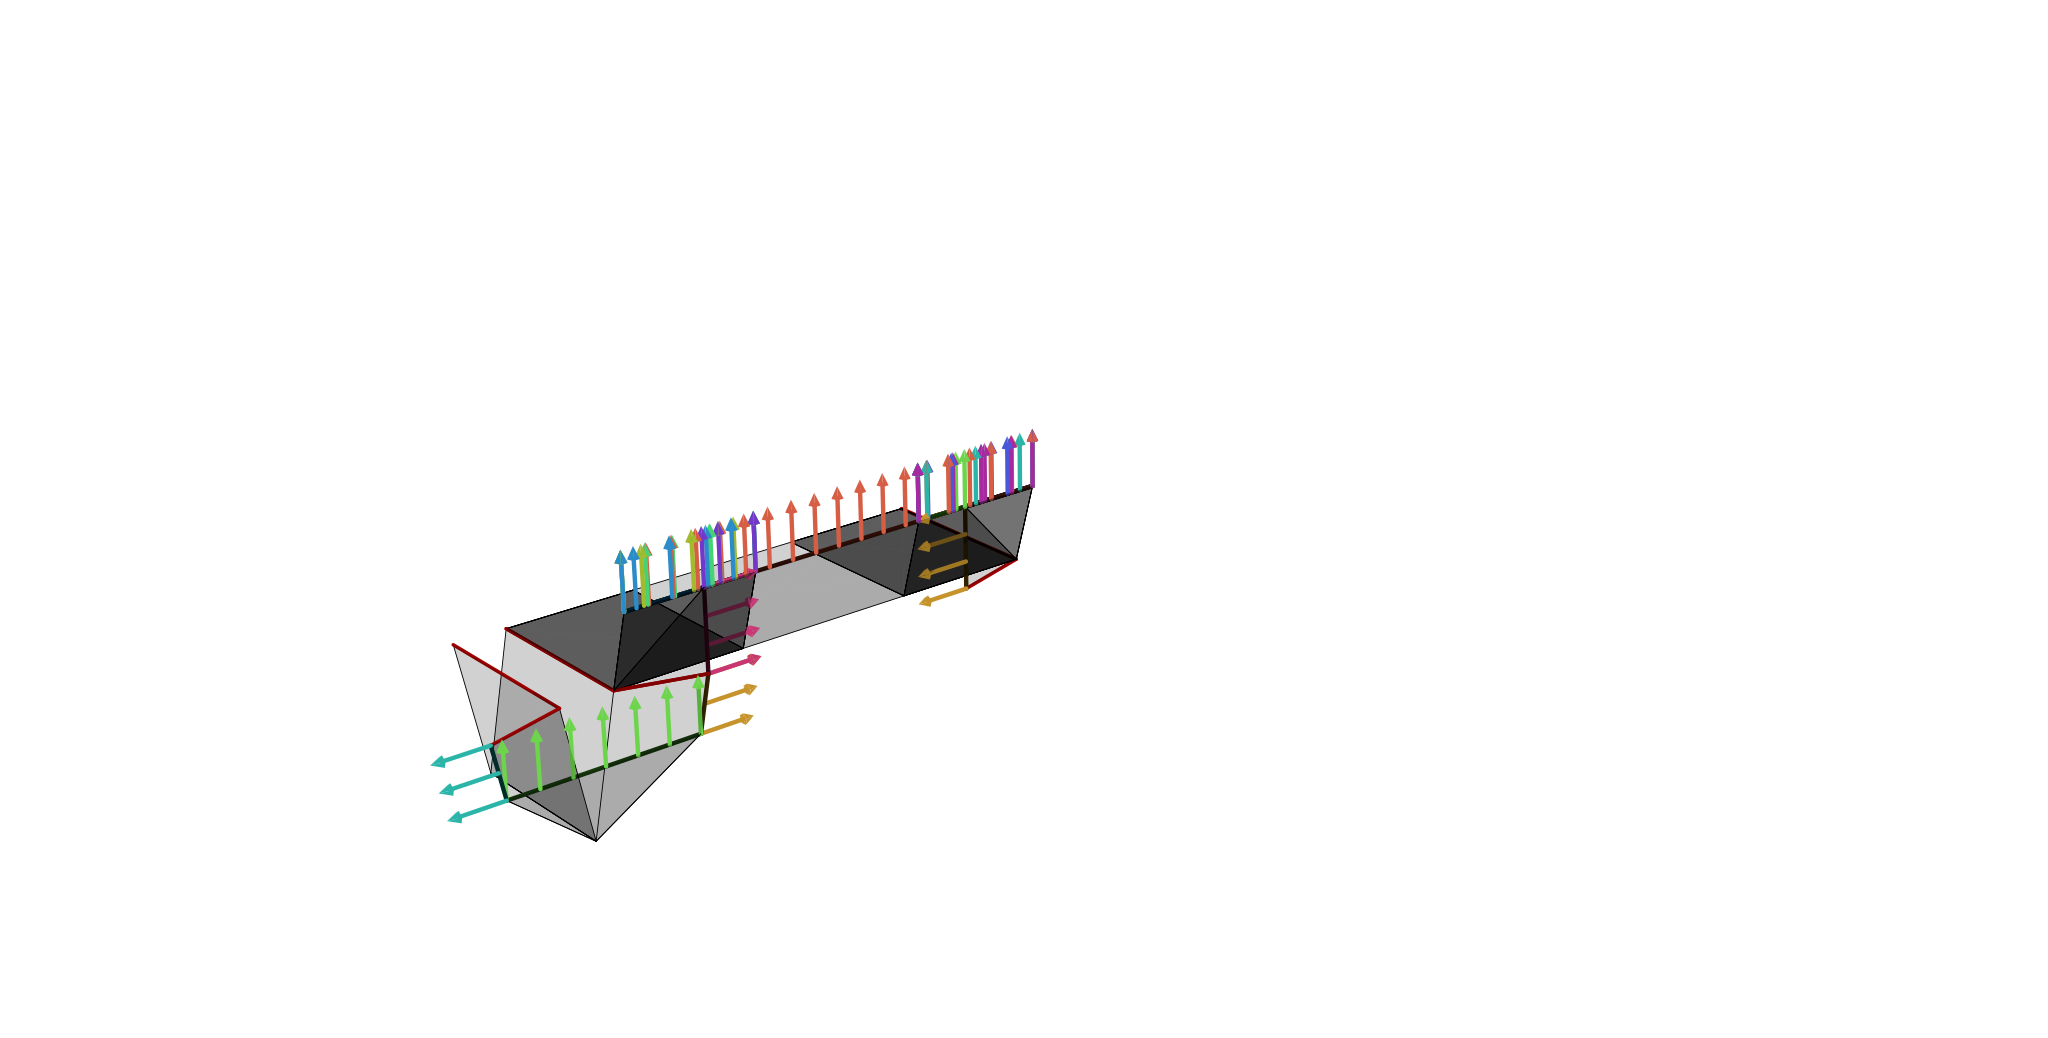
\includegraphics[width=0.21\textwidth]{figures/column_connector/column2.pdf}
    }%
    \subfloat[Connector at maximum width.]{
        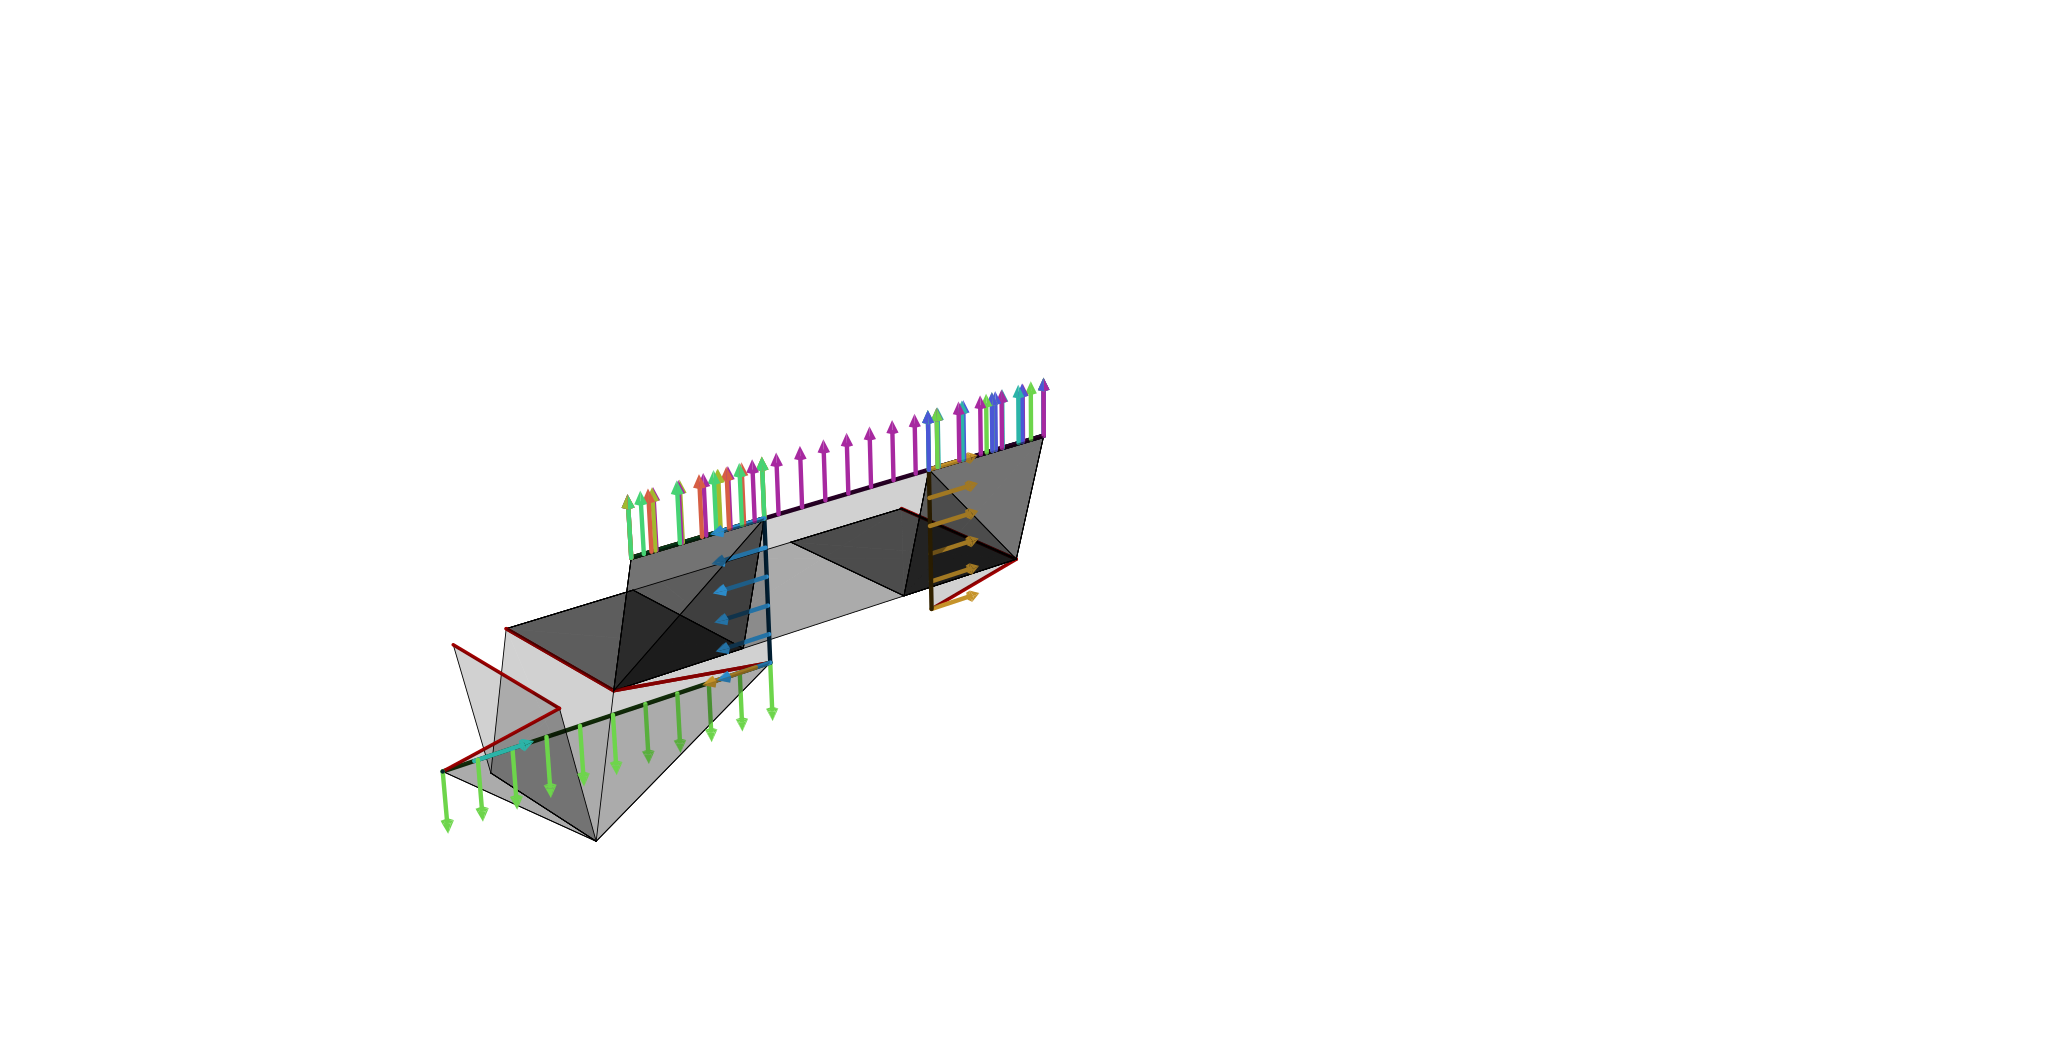
\includegraphics[width=0.24\textwidth]{figures/column_connector/column3.pdf}
    }%

    \subfloat[Connector moves inwards.]{
        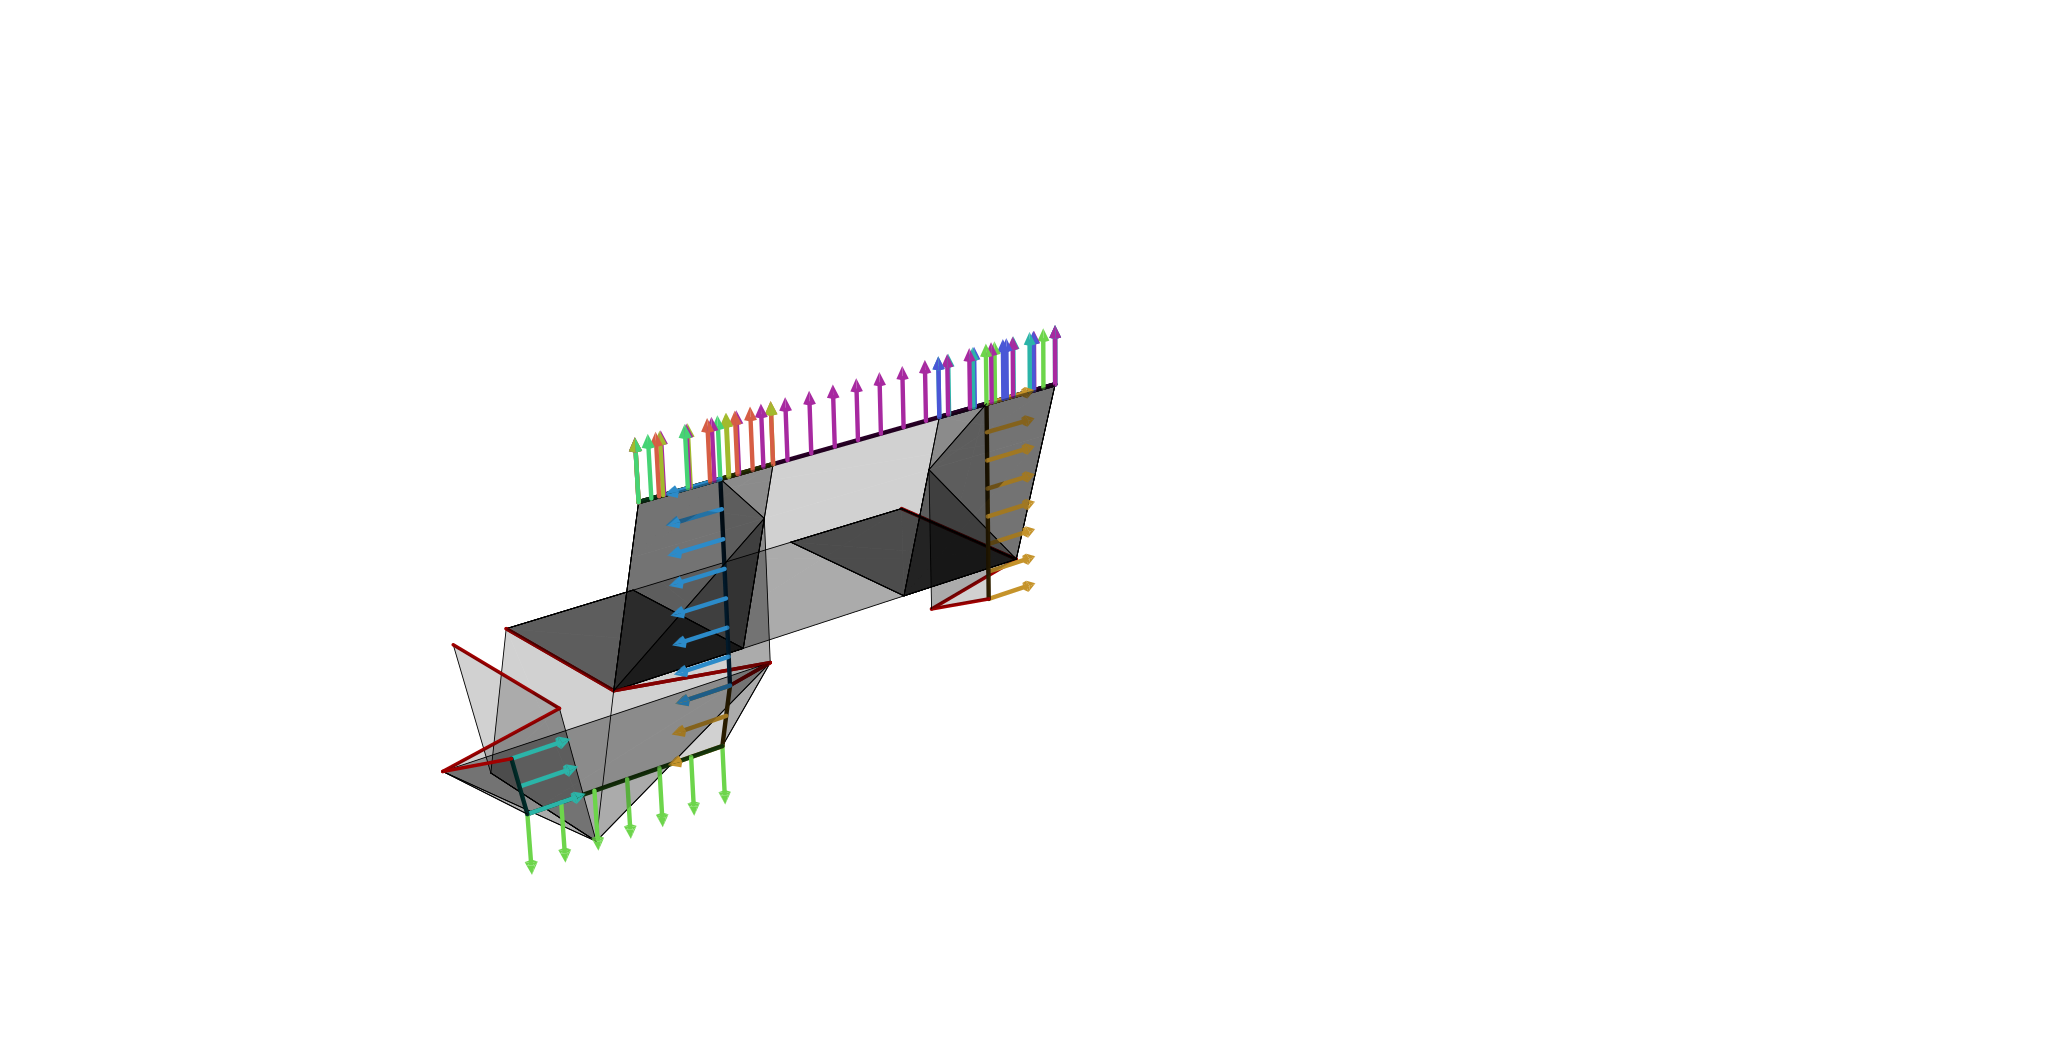
\includegraphics[width=0.23\textwidth]{figures/column_connector/column4.pdf}
    %}
    %\subfloat[]{
        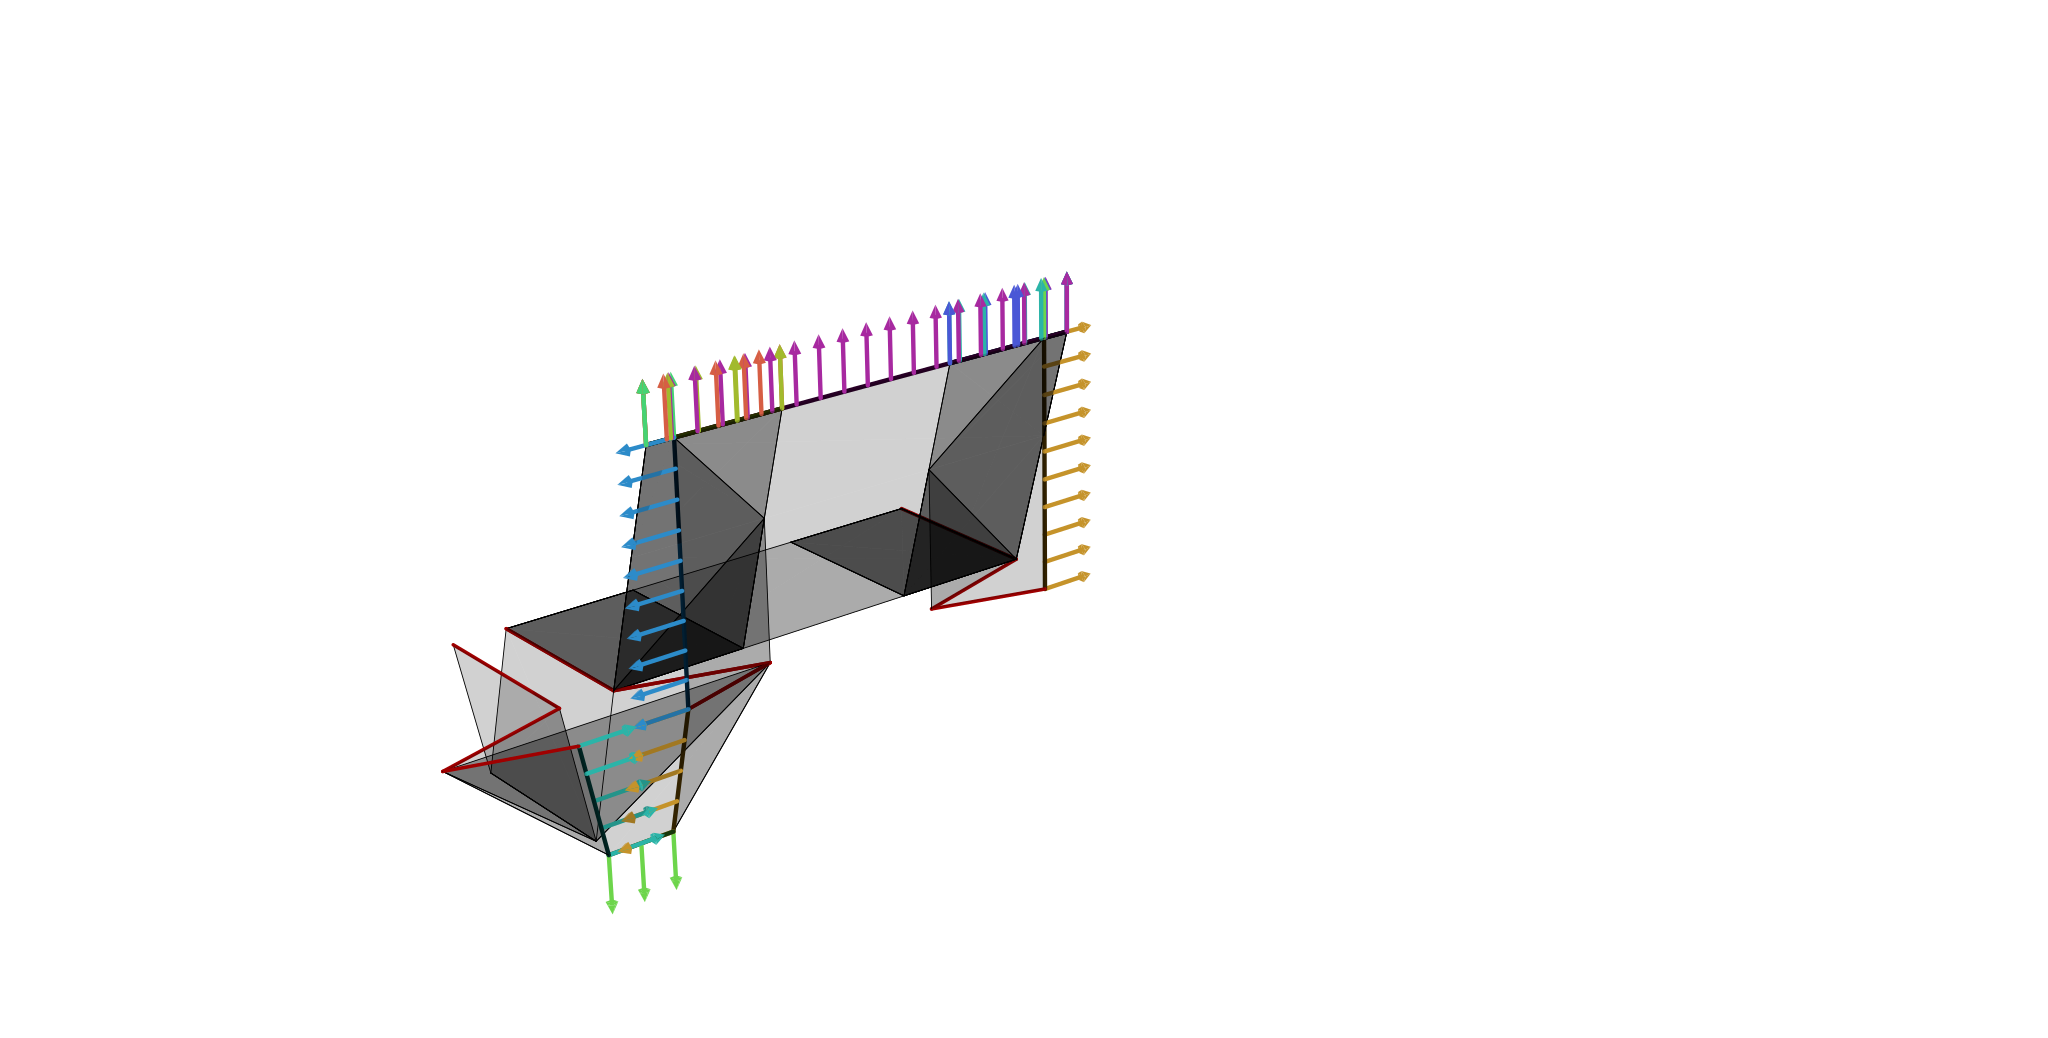
\includegraphics[width=0.23\textwidth]{figures/column_connector/column5.pdf}
    }%
    \subfloat[Back to \textbf{(a)}.]{
        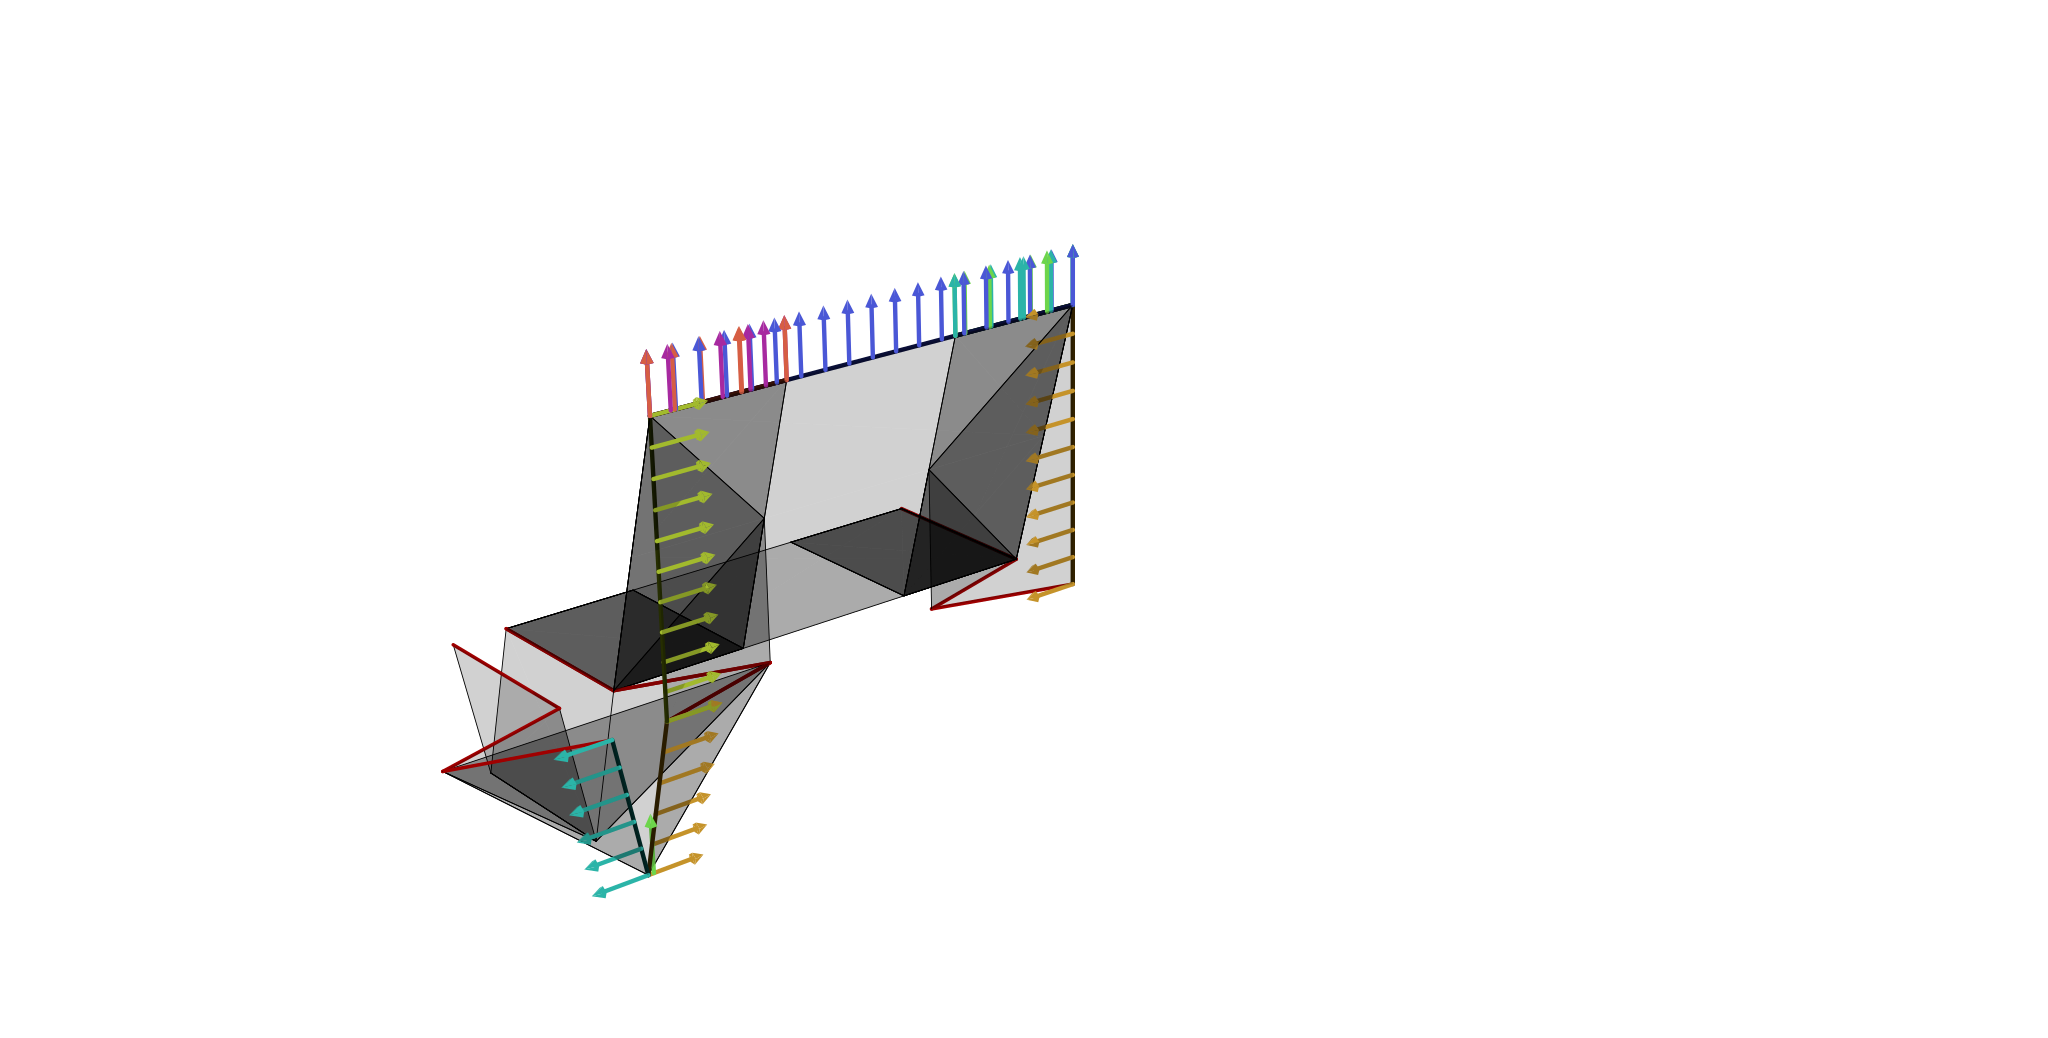
\includegraphics[width=0.23\textwidth]{figures/column_connector/column6.pdf}
    }%
    \subfloat[Same as \textbf{(b)}.]{
        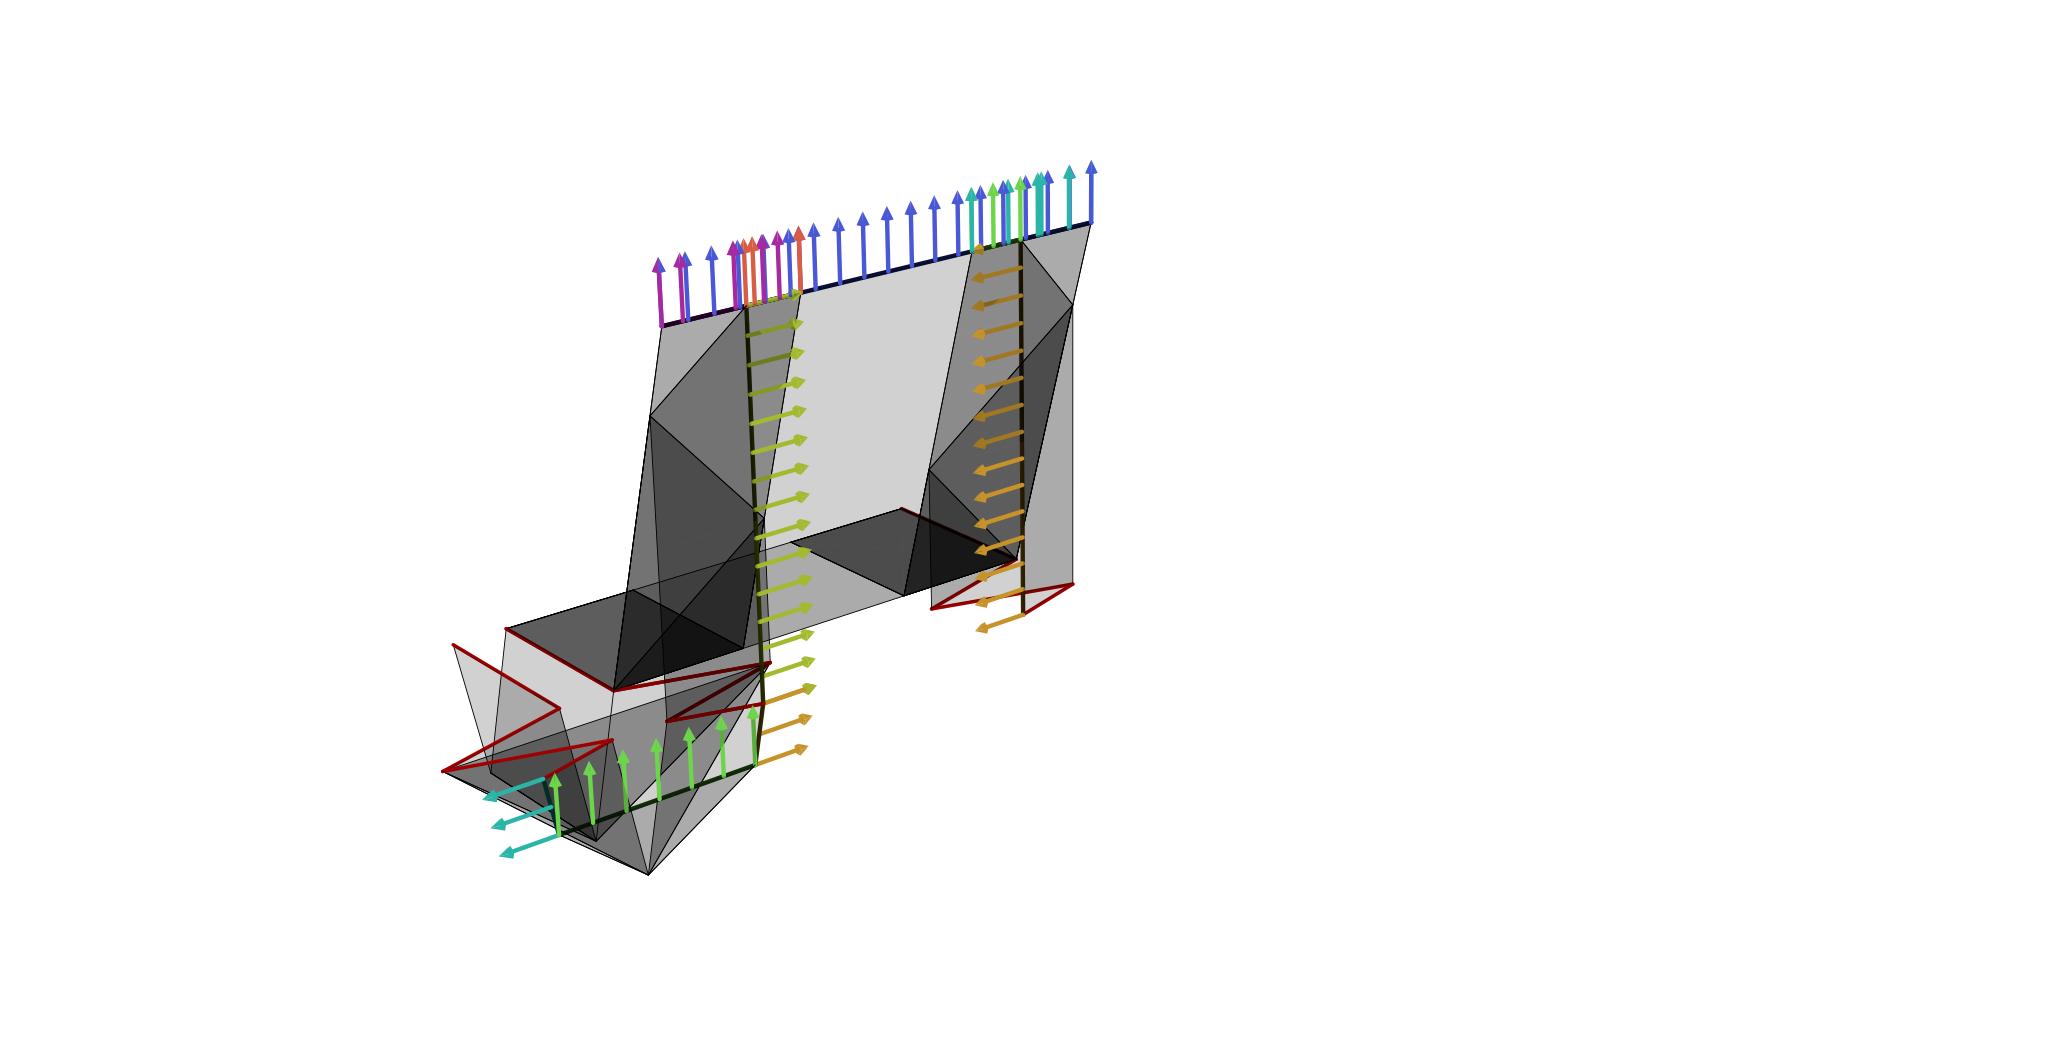
\includegraphics[width=0.23\textwidth]{figures/column_connector/column7.pdf}
    }%

    \subfloat[Same as \textbf{(d)}.]{
        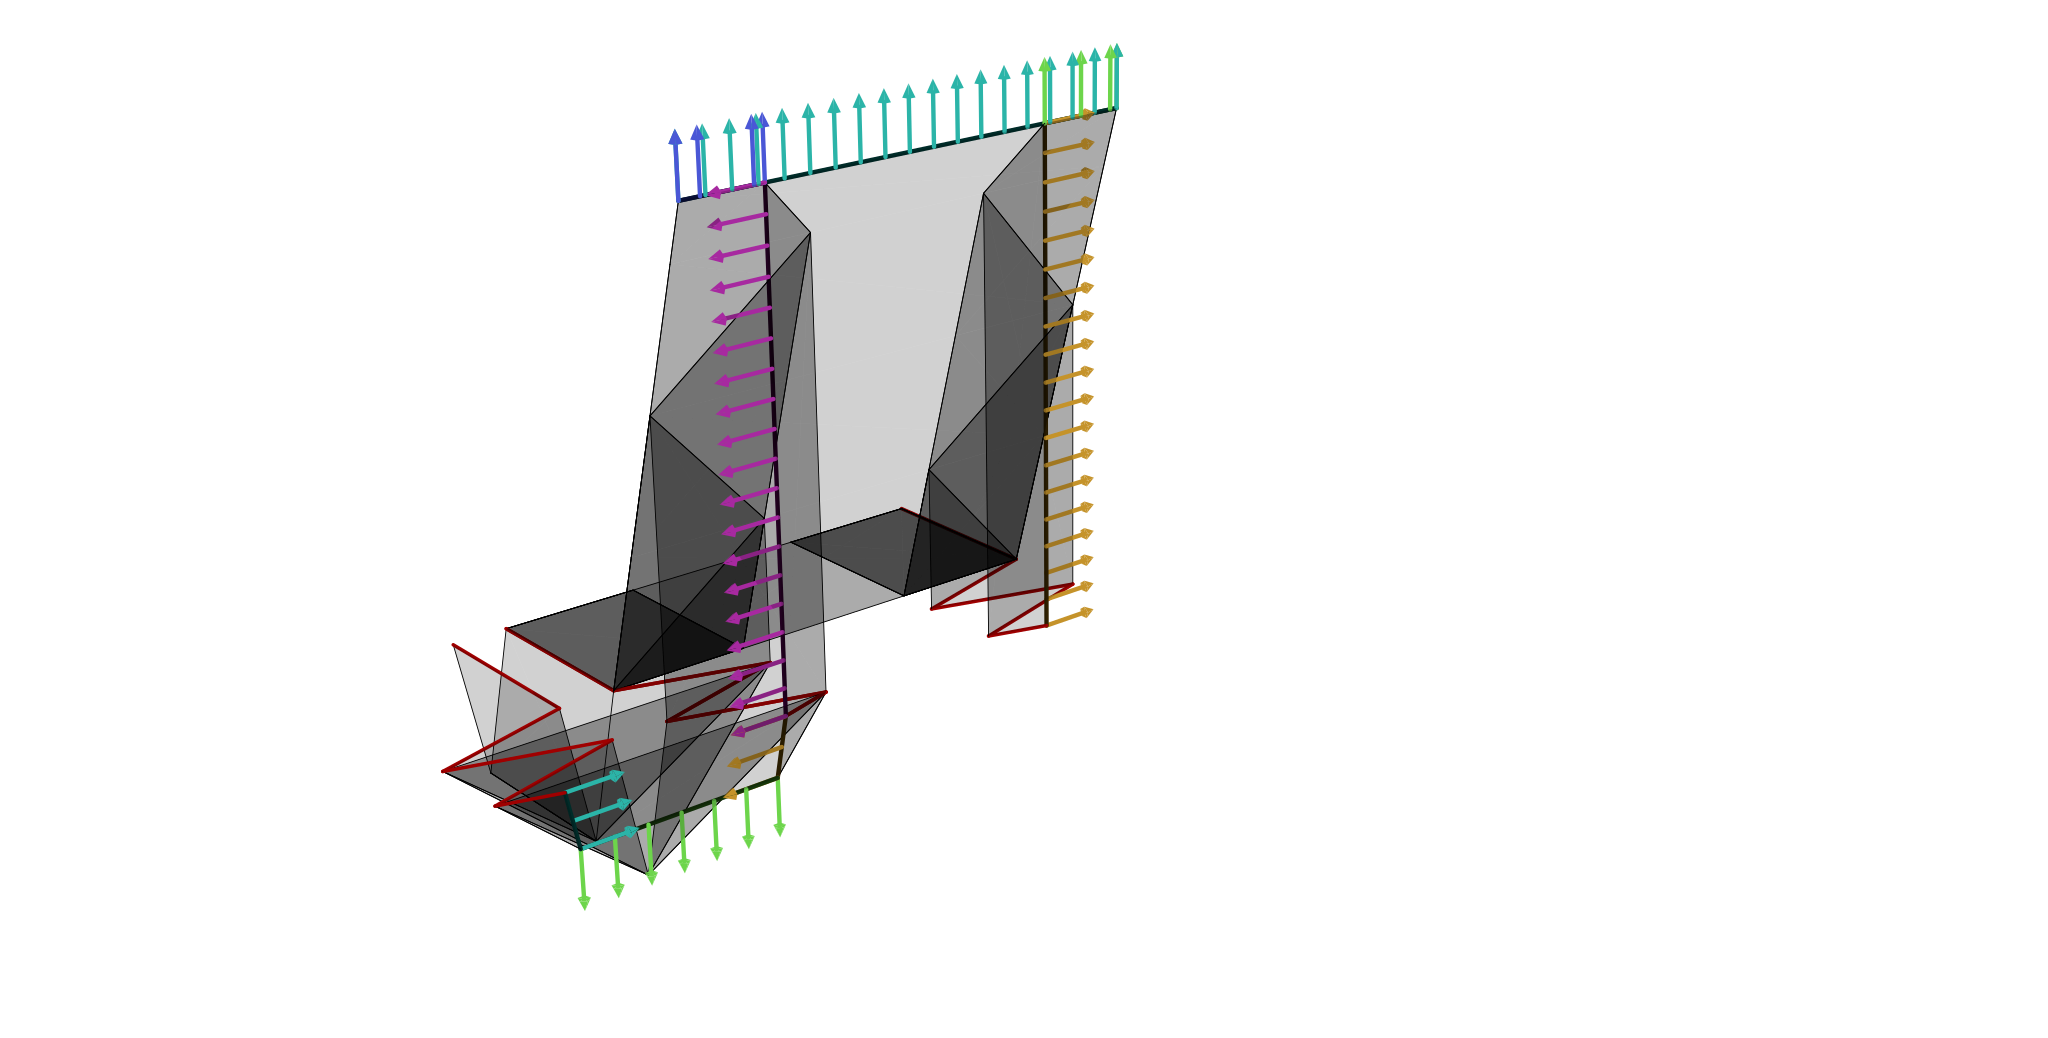
\includegraphics[width=0.29\textwidth]{figures/column_connector/column8.pdf}
    }%
    \subfloat[Level shift complete, and next level continues.]{
        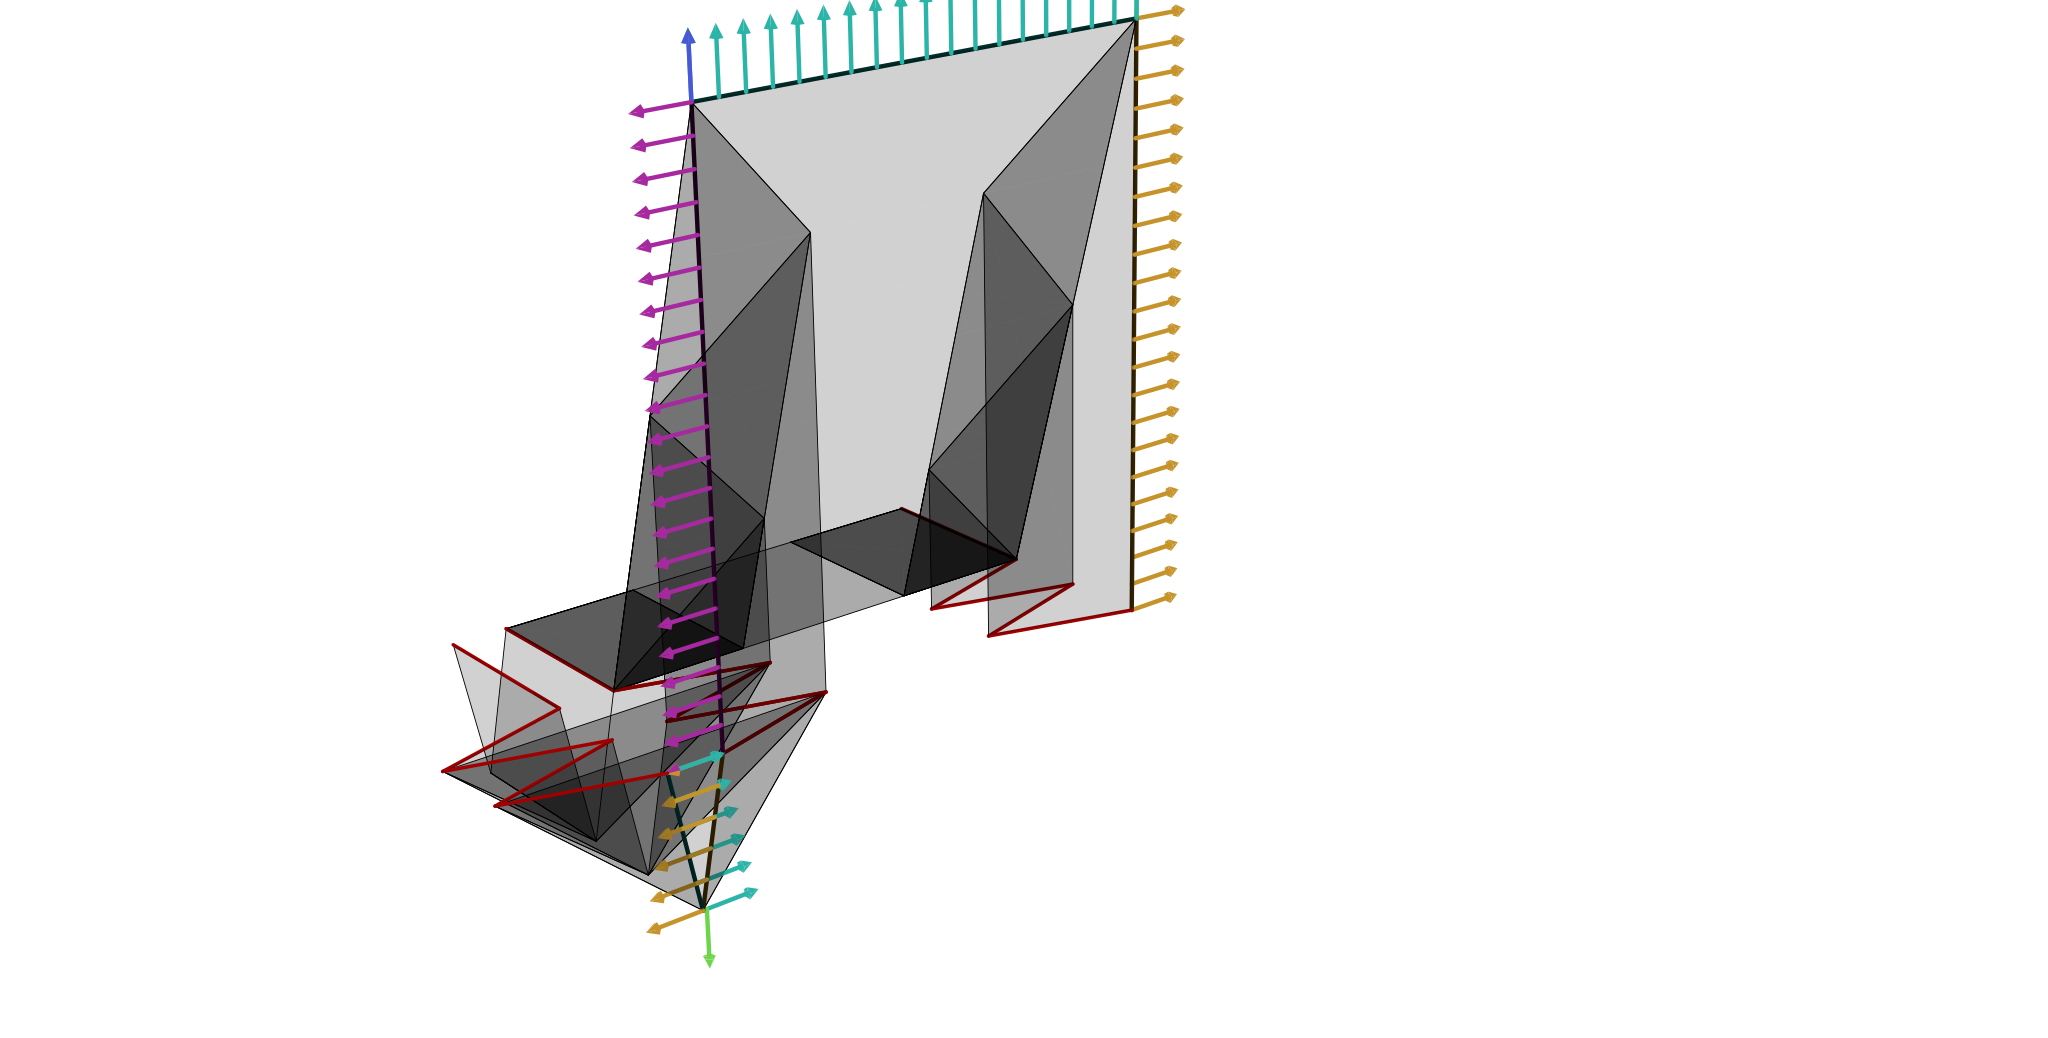
\includegraphics[width=0.29\textwidth]{figures/column_connector/column9.pdf}
    %}
    %\subfloat[Column and connector]{
        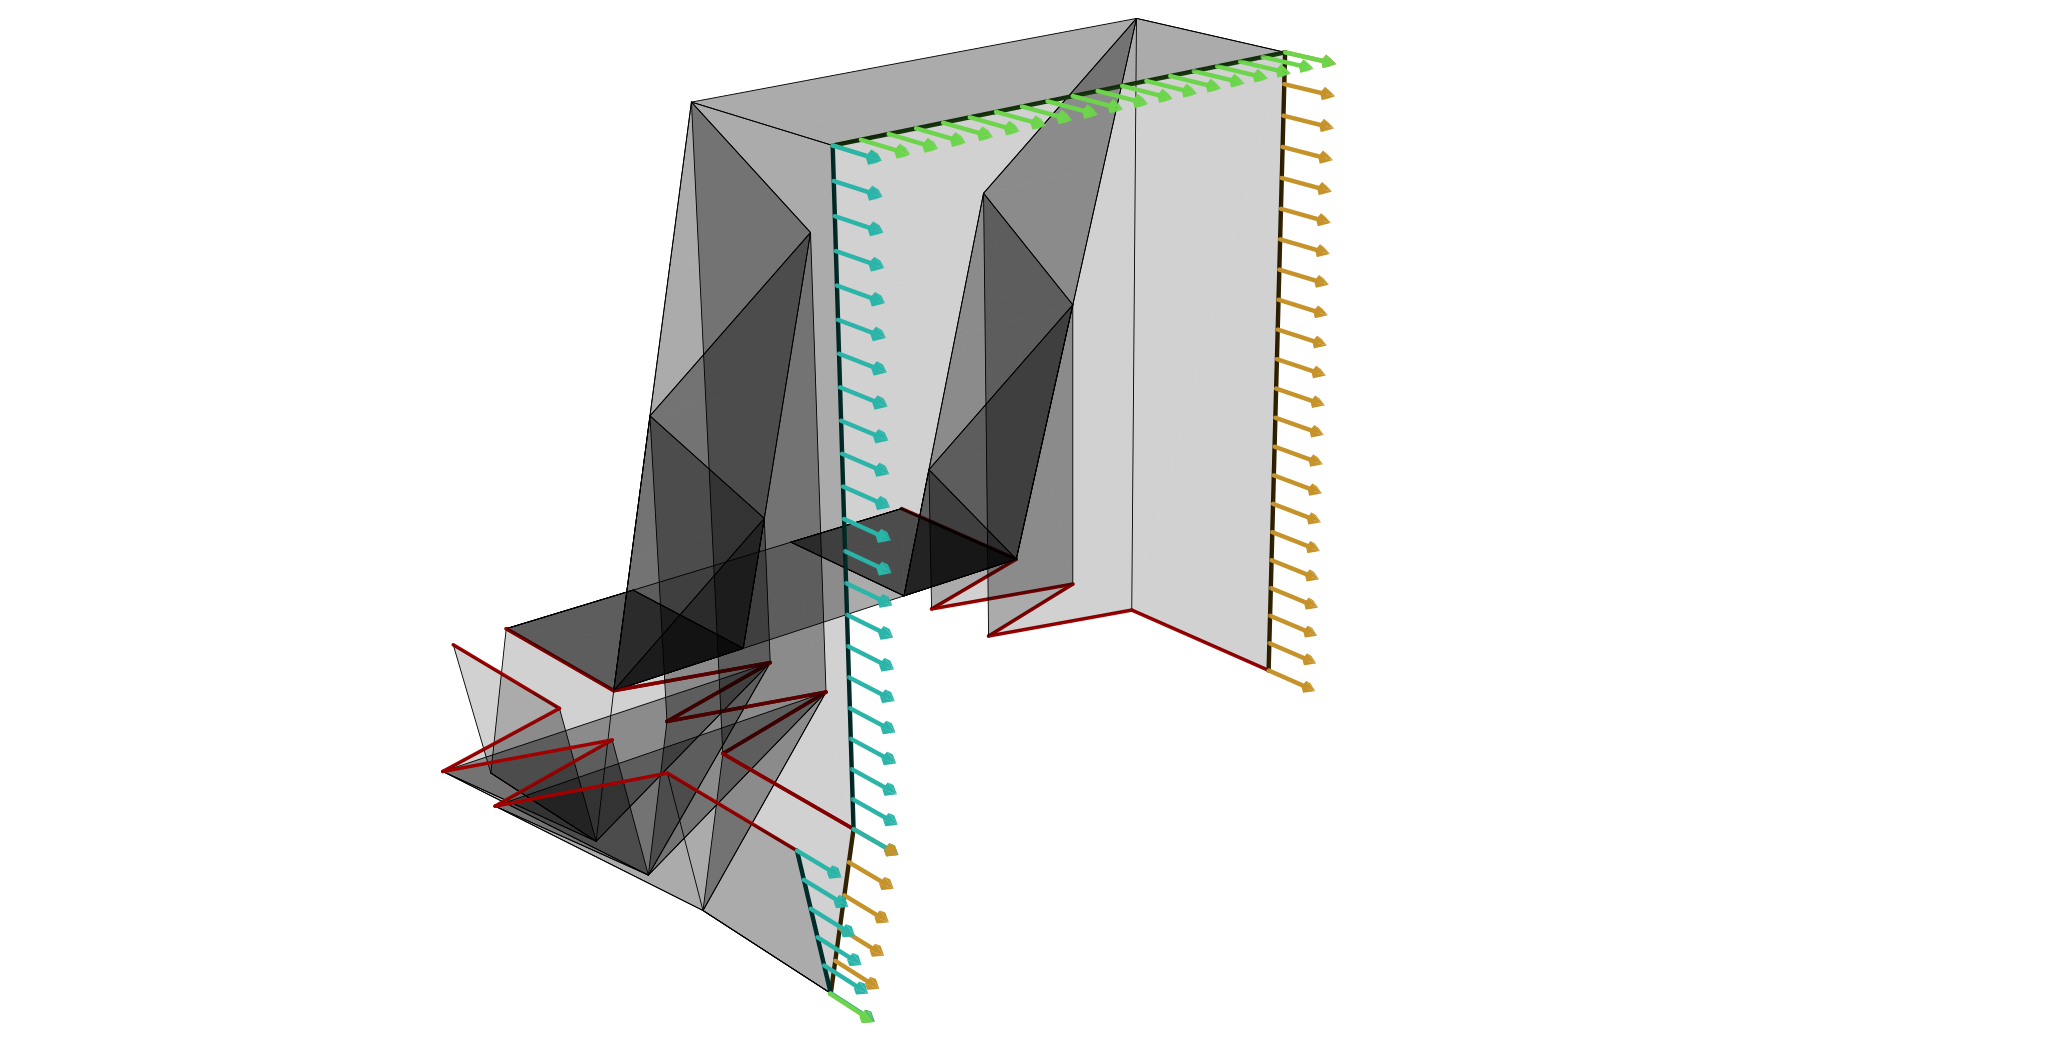
\includegraphics[width=0.34\textwidth]{figures/column_connector/column11.pdf}
    }%

    \subfloat[Connector gadget.]{
        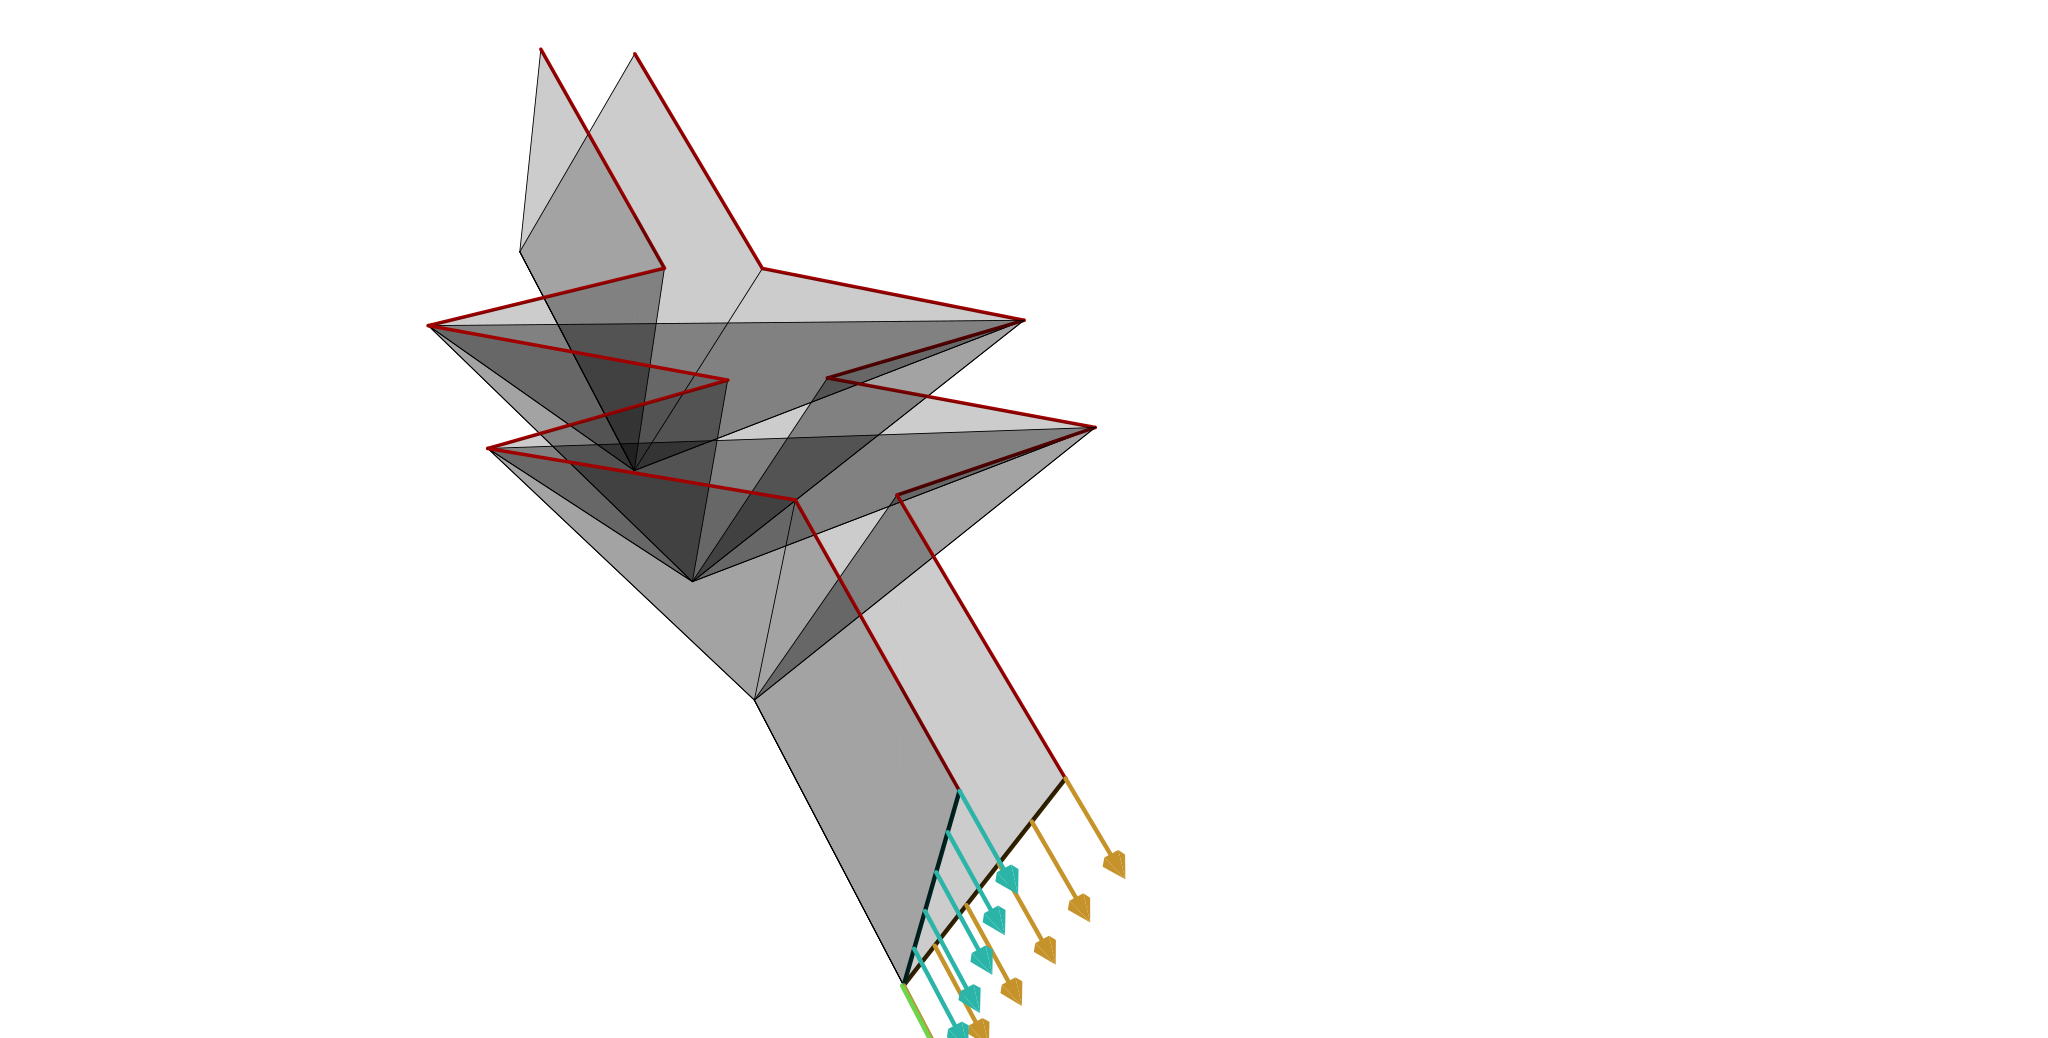
\includegraphics[width=0.31\textwidth]{figures/column_connector/connector0.pdf}
    }%
    \subfloat[Side view.]{
        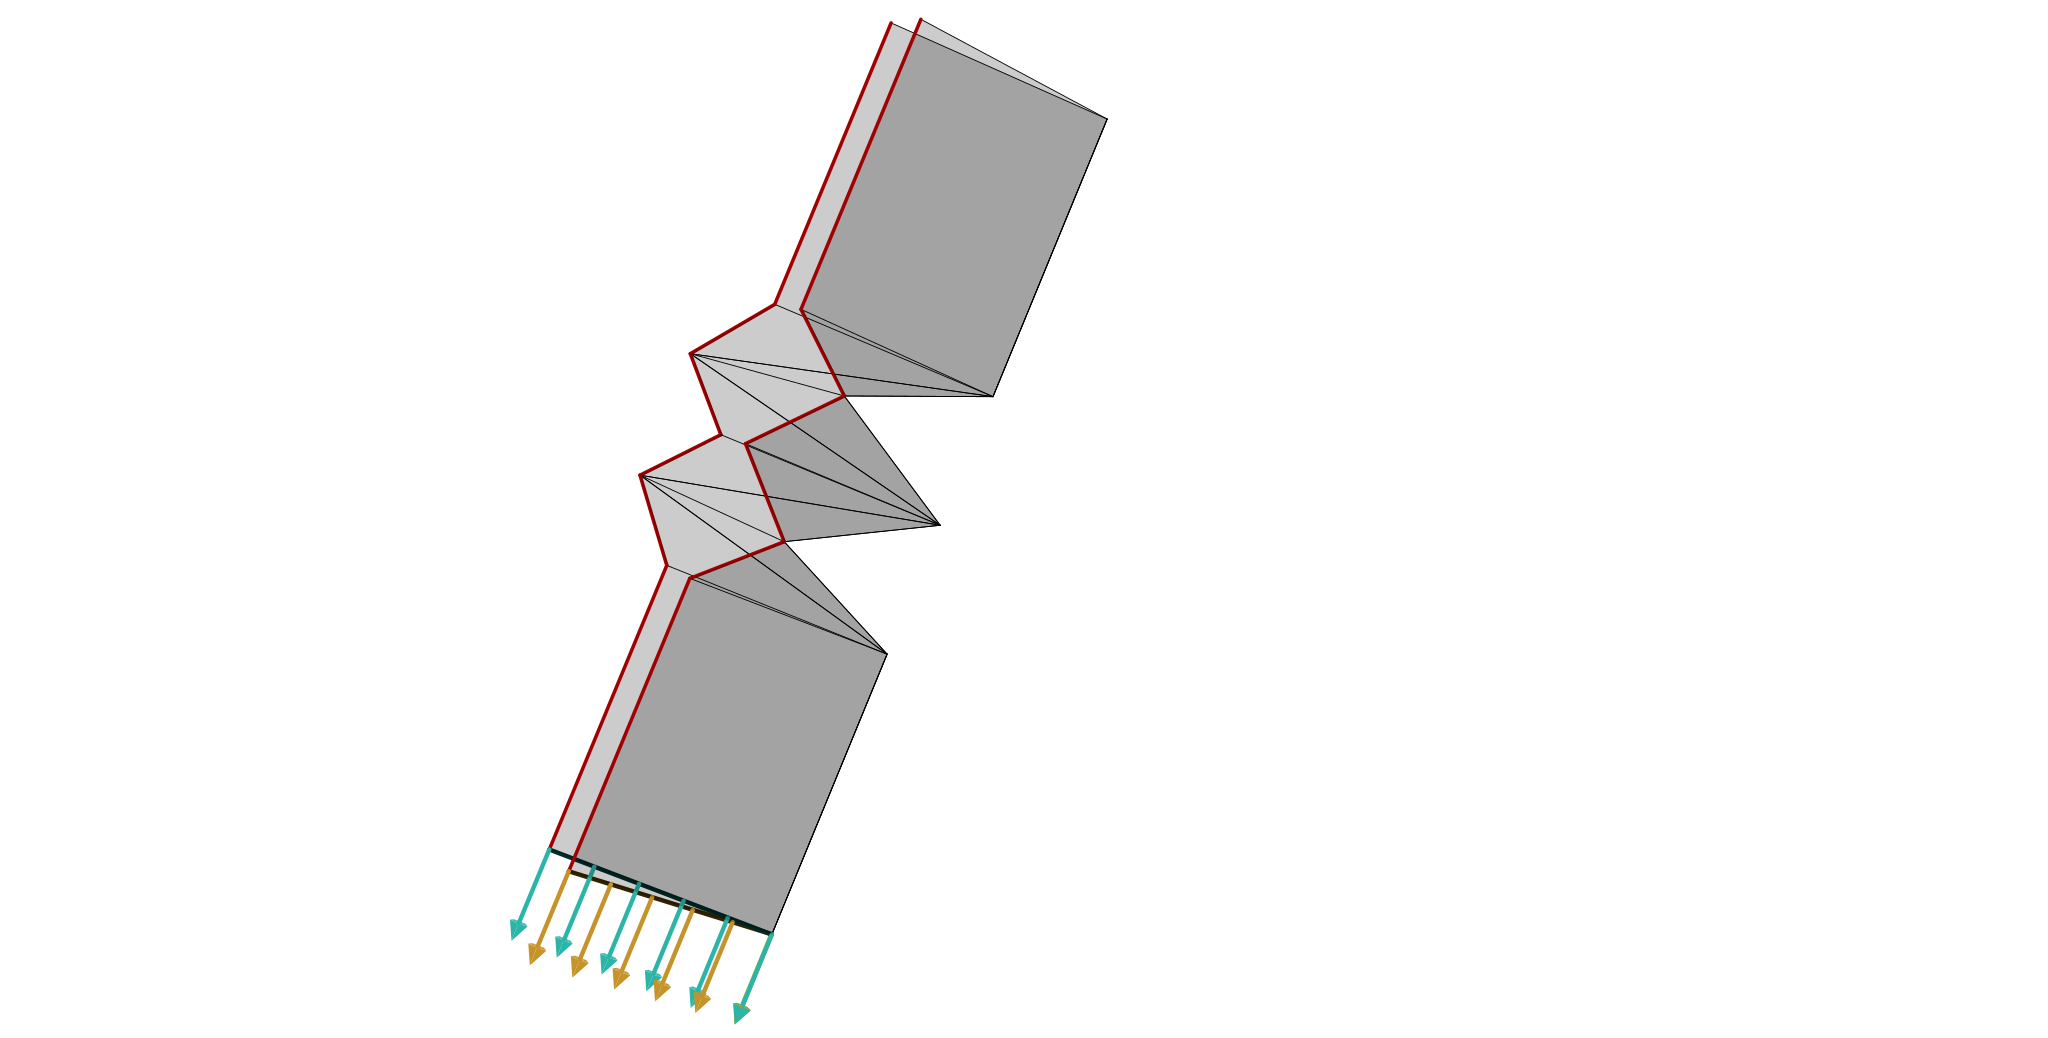
\includegraphics[width=0.27\textwidth]{figures/column_connector/connector1.pdf}
    }%
    \subfloat[Flat folded state.]{
        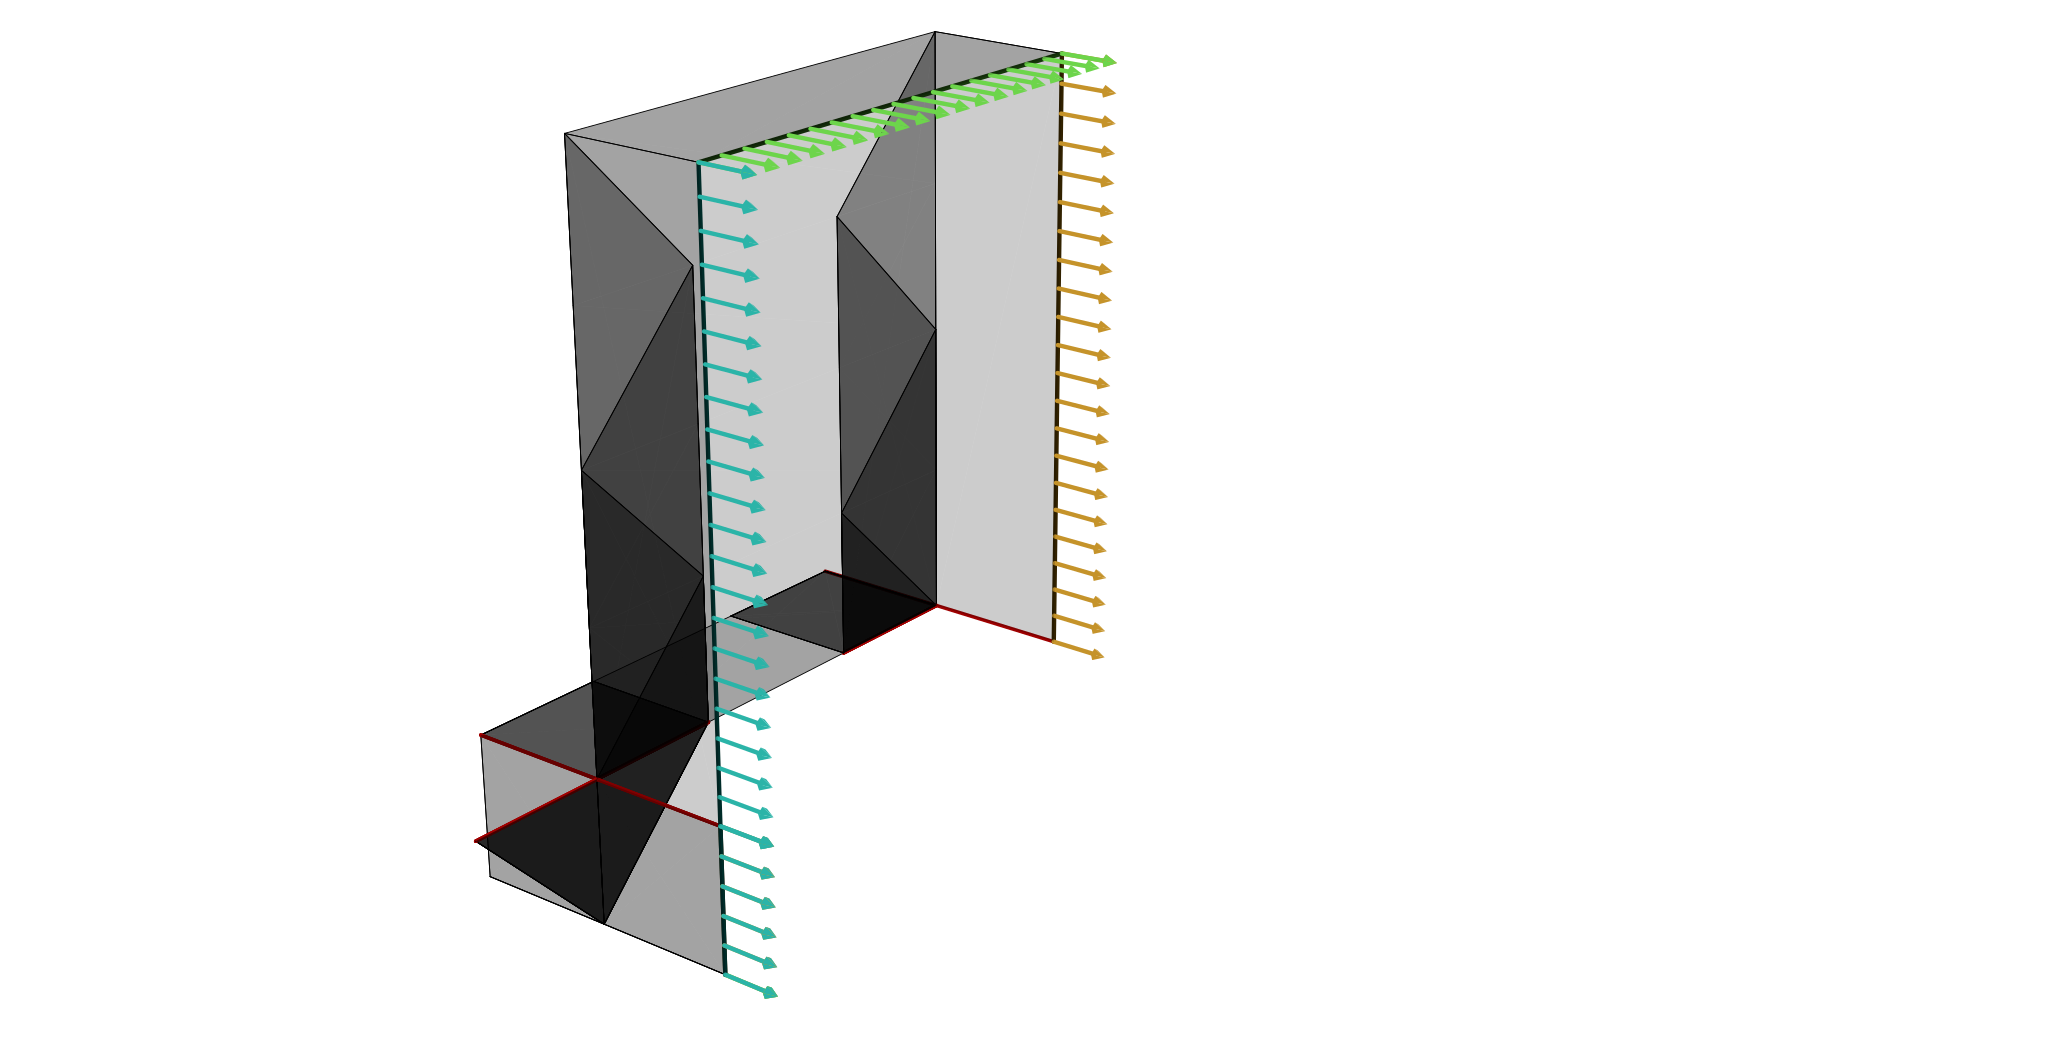
\includegraphics[width=0.31\textwidth]{figures/column_connector/column_connector0.pdf}
    }%
    \caption{
    Column gadget attached to a single column connector gadget.
    The red line demarcates the interface between the two gadgets.
    }
    \label{fig:column_connector}
    \vspace{-20pt}
\end{figure}
\clearpage


%\subsubsection{Alignment with Level Shifts}
%\label{sec:alignment_with_level_shifts}



\subsection{Size of Construction}
\label{sec:size}

From Proposition~\ref{prop:accordion_layers}, we know that each column extrusion strip
$\mathcal C^{(i)}$ has width $\left( 1 + 2\cdot\max_j\left\{ E_{ij}\right\}\right)$.
Additionally, we have $n-1$ strip connecors, each of width $2\varepsilon$.
We define $M_i = \max_j\left\{ E_{ij}\right\}$. So, the total width of the orthogonal terrain construction is
$$X = 2(n-1)\cdot\varepsilon + n + 2\cdot\sum\limits_{i=1}^n M_i$$
Now, note that our construction is also valid for any $\varepsilon' = \varepsilon/(2k)$, where $k$ is an integer.
In other words, we can make $\varepsilon$ arbitrarily small.

\begin{theorem}
\label{thm:grid_extrusion}
Using the time evolution ($y$ dimension) from Proposition~\ref{prop:accordion_layers},
we conclude that a grid extrusion can be folded from a strip of size $X\times T$, where
\begin{align}
X = n + 2\cdot\sum\limits_{i=1}^n M_i + o(1) && T = m + \sum\limits^{m-1}_{j=1} D_j
\end{align}
\end{theorem}

\subsection{Removing the Zero Level Assumption}
\label{sec:zero_level_assumption}


\subsection{Worst-Case Efficiency}
\label{sec:optimality}

Consider an $n\times n$ orthogonal terrain where the highest points along $x$-axis are $M = \max_j E_{ij}$,
and the maximum deltas along the $y$-axis are $D_j = \max_i{\|E_{i,j}-E_{i,j+1}\|} = M$.
For example, one such ``worst-case'' orthogonal terrain is the following
checkerboard alternating between the minimum and maximum heights:
$$
E_{ij}=
\begin{cases}
M & \textrm{ if $(i+j)$ is even,}\\
0 & \textrm{ if $(i+j)$ is odd.}
\end{cases}
$$

We assume that the top faces of the terrain form axis-aligned squares in the unfolded state,
The longest line formed along either axis is the total length of the top surfaces plus the sum of the height changes across the axis, which gives
$$L = n + \sum^{n}_{i=1} M = n + (n-1)\cdot M.$$
We conclude that the minimum required size of a folding is $L\times L$.

From Theorem~\ref{thm:grid_extrusion}, we know that the terrain can be folded from an $X\times Y$ strip of paper,
where $X = n + 2(n-1)\cdot M + o(1)$ and $Y = n + (n-1)\cdot M$.
Since $Y = L$, and $X < 2L$ (assuming an appropriately small value of $\varepsilon$),
our construction results in a folding that is within a factor two of the optimal paper usage for this terrain, under the aforementioned assumption.

%\begin{claim}
%The $x$-axis length of the strip of paper required to fold this shape can be made arbitrarily close to $X$.
%\end{claim}
%\begin{claim}
%The $y$-axis length of the strip of paper required to fold this shape will be exactly $Y$.
%\end{claim}

%First, we pick an $\epsilon$, such that $2\varepsilon$ divides all extrusion heights.
%The construction will require paper of size $X'\times Y$, where $X' = X + 2\epsilon(n-1)$.

%There are two components to the construction
%\begin{itemize}
	%\item $n$ strips parallel to the $y$-axis. Each of these strips will fold to the corresponding strip in the extruded graph. The total area of these strips will be $X\times Y$.
    %\item $n-1$ Intermediate strips, each of size $2\epsilon\times Y$ to connect the main strips together.
%\end{itemize}
%The total area is therefore $X\times Y + (n-1)2\epsilon\times Y = X'\times Y$. This can of course be made arbitrarily close to $X\times Y$.


